\subsection{External Interface Requirements}
\subsubsection{User Interfaces}
The user application has to be developed, as stated numerous times, for every kind of demographics.
This includes visually impaired users and people not familiar with modern technologies.

Hence, the interface must:
\begin{enumerate}
    \item remain simple on every page and menu
    \item follow standards in design to accomodate users into finding which are the interactible parts of the application; for example Material Design by Google and/or Apple iOS design standards could be applied
    \item communicate via short and concise messages
    \item show important information without having to navigate multiple times into sub-menus
    \item integrate correctly with OS screen reader technologies to be usable by blind people
    \item use an adaptive layout to support devices with different resolutions and aspect ratios
\end{enumerate}

\subsubsection{Hardware Interfaces}
CLup software runs on different platforms and different kinds of hardware depending on the part of the system services it is required to run.

To run the CLup mobile application it is required a device with mobile internet access (e.g. a smartphone or a tablet) and at least 1GB of ram (to be able to not experience lags due to memory used by other applications). Most of today's smartphones start with 2GB of RAM anyway.
GPS is used to retrieve the current location but can be replaced with manual insertion of the needed data by the user.

Automation systems communicating in a LAN do not have specific requirements: many different solutions can be employed and can vary from different kind of store. The store main system must be able to communicate with the CLup APIs, and it is required to have a working internet connection.

CLup main servers on the other hand can exploit newest standards on Serverless computing, modularizing functions in microservices and be able to keep up with an increase of requests and stores adopting the S2B.
\vfill


\subsubsection{Software Interfaces}
CLup will expose REST APIs in order to exchange data from a local store server to CLup main servers.

Automation systems will communicate with the local store server without any constraints, even though standard REST APIs for internal information exchange will also be provided by the S2B.

\subsubsection{Communication Interfaces}

Connections from remote to local servers will be done over TCP/IP and HTTPS.
CLup REST API's will require valid tokens to verify authentication.

Local subsystems interfacing with the local main server should be connected to a private Intranet to lower the risk of possible cracking attempts.

Local subsystems can also be developed and connected with IoT standards, for example employing communication through protocols like MQTT.

\subsection{Functional Requirements}
\subsubsection{Use cases}
Here is a list of relevant use cases for the S2B. These use cases are also shown in the figure \ref{fig:Use_Case_Diag}
\smallskip

\rowcolors{2}{gray!25}{white}
\renewcommand{\arraystretch}{1.4}
\captionof{table}{Use Cases table}
\begin{tabular}{C{2cm}L{10.5cm}C{2.6cm}}
    \rowcolor{gray!50}
    Label & Use Case                                                                                          \\
    UC1   & Customer Registration                                                                             \\
    UC2   & Customer/Operator Authentication                                                                  \\
    UC3   & Customer search for the store page                                                                \\
    UC4   & Customer adds/removes a store from their favorites list                                           \\
    UC5   & Customer books a visit in a store                                                                 \\
    UC6   & Customer creates/edits a shopping list                                                            \\
    UC7   & Customer creates a numbered virtual ticket to enter a store as soon as there is a place available \\
    UC8   & Customer creates a physical numbered ticket                                                       \\
    UC9   & Customer cancels a previously created ticket                                                      \\
    UC10  & Customer scans the ticket through an access control system to enter                               \\
    UC11  & An user leaves the store through an exit with a people counter installed                          \\
    UC12  & A store operator checks statistics about the store                                                \\
    UC13  & User resets his password                                                                          \\
\end{tabular}
\medskip
\begin{figure}[H]
    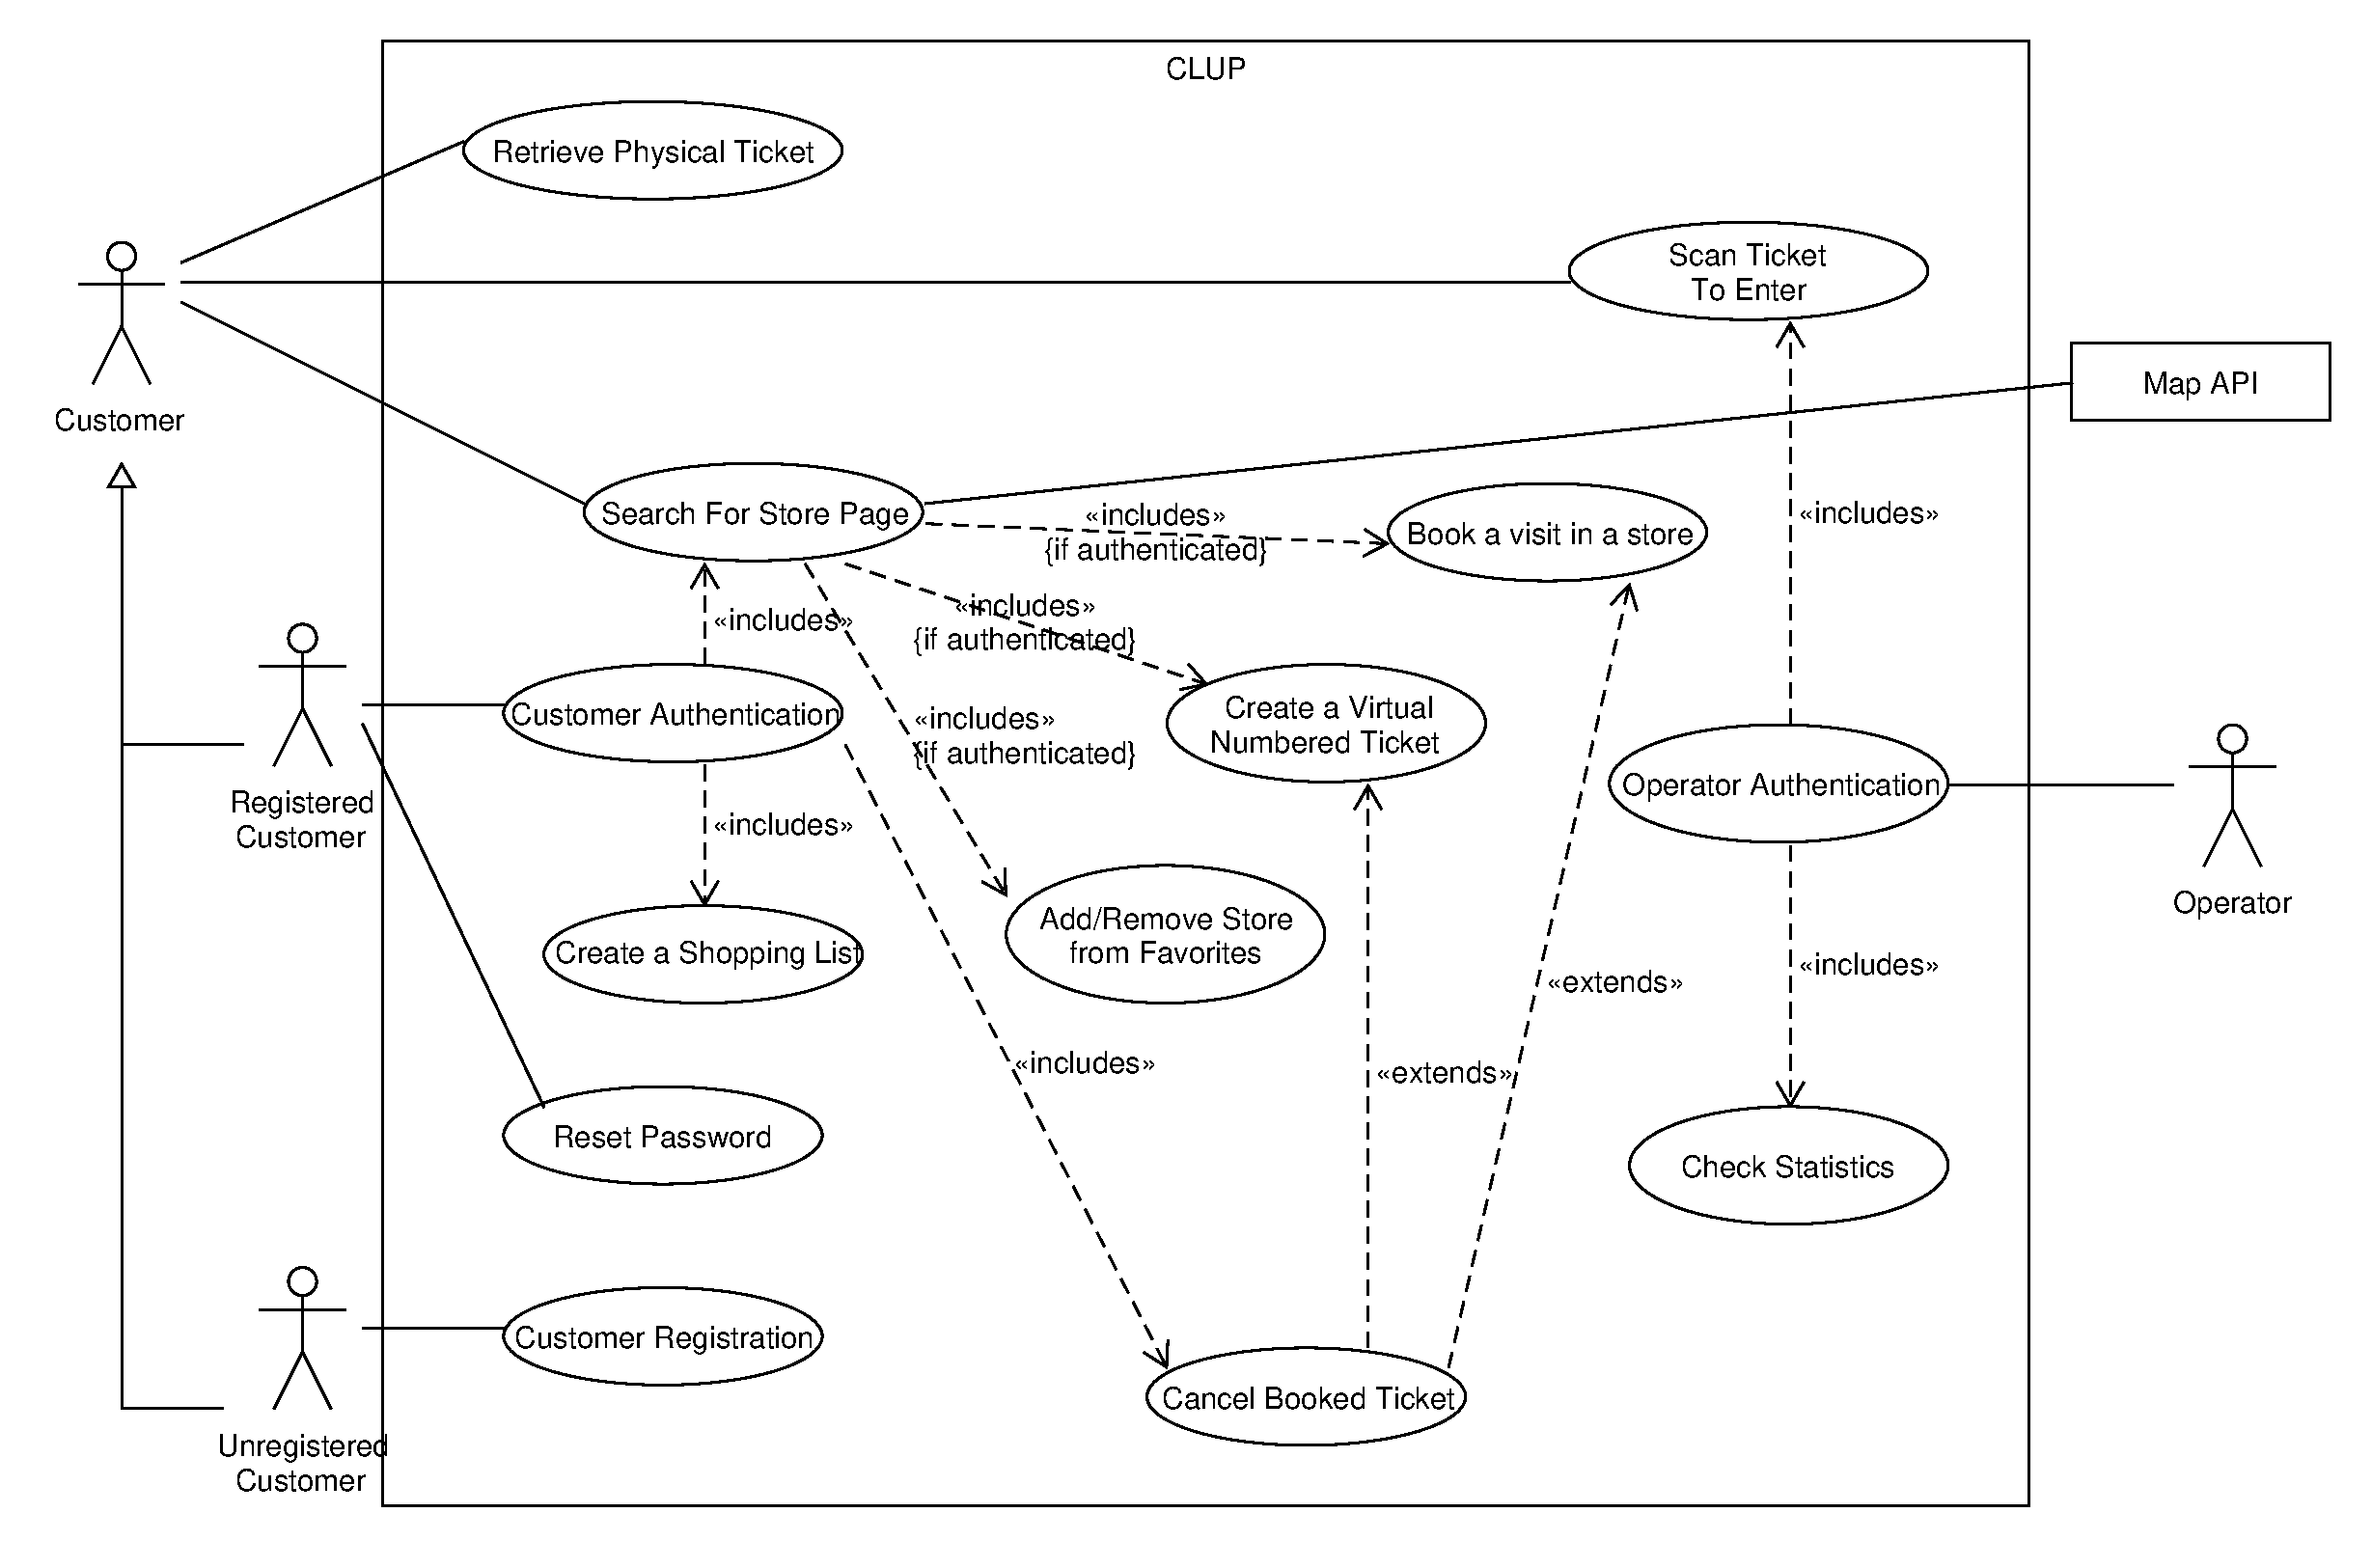
\includegraphics[width=\textwidth]{Images/UML_use_case.pdf}
    \caption{\label{fig:Use_Case_Diag}Use Case Diagram for the S2B}
\end{figure}


\medskip
\clearpage
% COuld be useful to report this on the dictionary section on chapter 1%
In the following use case description tables, if not explicitly stated otherwise, the term ``user'' is used interchangeably with the term ``customer''.
\medskip

\textbf{Use case 1: User Registration}
\smallskip

\rowcolors{1}{white}{white}
\begin{longtable}{p{0.25\linewidth}p{0.75\linewidth}}
    \toprule
    \textbf{Name}             & \textbf{User Registration}                                                                                                        \\
    \midrule
    \textbf{Actors}           & Unregistered customer                                                                                                             \\
    \midrule
    \textbf{Entry conditions} & The user requests the system to register                                                                                          \\
    \midrule
    \textbf{Flow of events}   &
    \begin{enumerate}
        \item The system shows the form with the required fields to register
        \item The user inserts his e-mail address and his password
        \item The user inserts his name, surname, birth date and his preferred home address
        \item The user is shown the recap of the information used to fill the form
        \item The user confirms the information, and the form is sent to the system
        \item The system sends a e-mail to the address provided by the user in the form. The e-mail contains a verification link
        \item The users open the e-mail and clicks on the verification link
        \item The system sends an e-mail to the user stating that their registration process ended successfully
    \end{enumerate}                                                                                                                                     \\
    \midrule
    \textbf{Exit conditions}  & The unregistered customer now is a registered customer and after authentication he can access all CLup customer functionalities \\
    \midrule
    \textbf{Exceptions}       &
    \begin{itemize}
        \item If the e-mail inserted is already registered in the system an error message tells the user that the provided e-mail is already in use by another account. The systems asks the user if they want to reset the password (See UC13 - User resets password) %TODO Add a link%
        \item While typing the password the system checks that the password is compliant with the password requirements listed in the section \ref{password_req}. If the password requirements are not met the system shows an error listing the non respected password requirements.
    \end{itemize}                                                                                                                                     \\
    \bottomrule
    \caption{\emph{Customer registration} use case description}
\end{longtable}

\begin{figure}[H]
    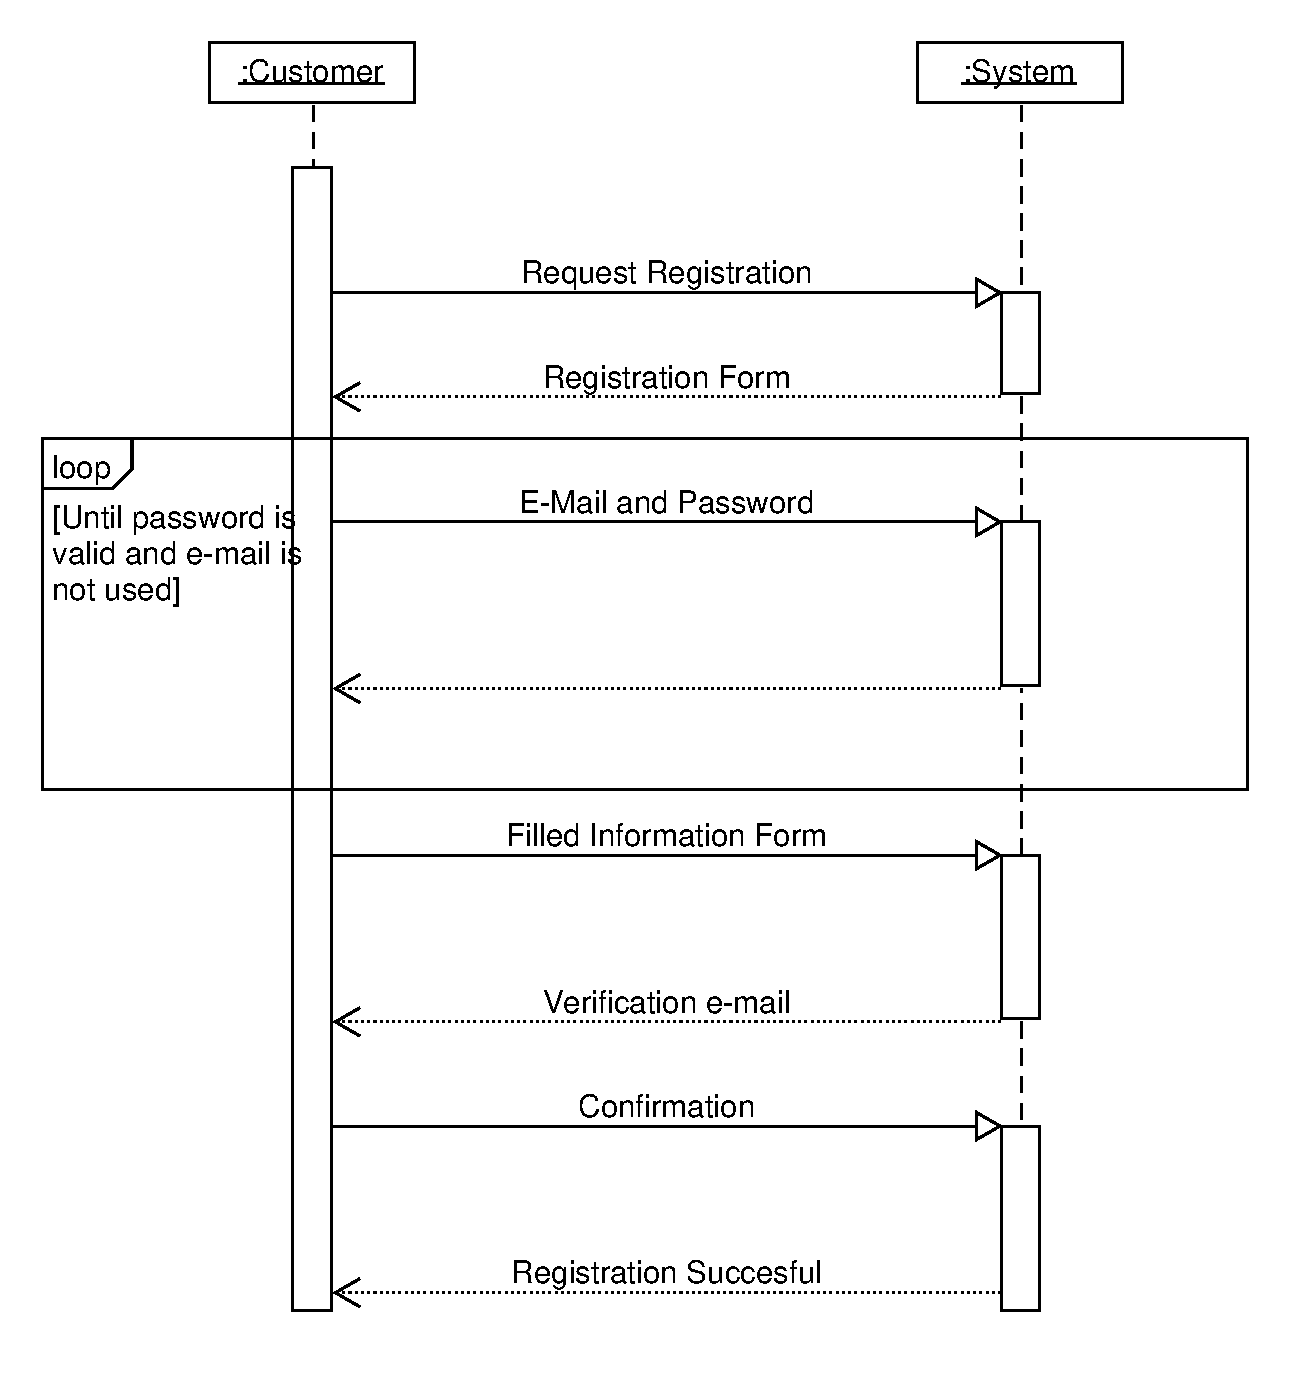
\includegraphics[width=\textwidth]{Images/UML_Seq_Diag_1.pdf}
    \caption{\label{fig:Use_Case_Diag}Sequence Diagram for Use Case 1}
\end{figure}

\clearpage
\textbf{Use case 2: User Authentication}
\smallskip
\rowcolors{1}{white}{white}
\begin{longtable}{p{0.25\linewidth}p{0.75\linewidth}}
    \toprule
    \textbf{Name}             & \textbf{User Authentication}                                                                                            \\
    \midrule
    \textbf{Actors}           & Registered Customer or Store Operator                                                                                   \\
    \midrule
    \textbf{Entry conditions} & The user requests the system to log-in                                                                                  \\
    \midrule
    \textbf{Flow of events}   &
    \begin{enumerate}
        \item The system shows the authentication form
        \item The user fills the form with his e-mail address used to register and his password
        \item The system checks if there is an account registered with the provided e-mail
        \item The system checks that the account's hashed password matches with the hashed password provided in the form
        \item The initial CLup page is shown to the user
    \end{enumerate}                                                                                                                           \\
    \midrule
    \textbf{Exit conditions}  & The user can use the CLup customer/operator application with all the functionalities available to authenticated users \\
    \midrule
    \textbf{Exceptions}       &
    \begin{itemize}
        \item If the e-mail or the password are incorrect then an error message is shown to the user
    \end{itemize}                                                                                                                           \\
    \bottomrule
    \caption{\emph{Customer authentication} use case description}
\end{longtable}

\clearpage
\textbf{Use case 3: Customer searches for store details}
\smallskip
\rowcolors{1}{white}{white}
\begin{longtable}{p{0.25\linewidth}p{0.75\linewidth}}
    \toprule
    \textbf{Name}                             & \textbf{Customer searches for store details}      \\
    \midrule
    \textbf{Actors}                           & Customer                                          \\
    \midrule
    \textbf{Entry conditions}                 & The user started the CLup customer application    \\
    \midrule
    \textbf{Flow of events}                   &
    \begin{enumerate}
        \item The system checks the position of the user with the GPS
        \item The system interfaces with an external map API downloading from it a map of the surroundings of the user position
        \item The system decorates the map with the positions of all store adopting CLup
        \item The system sends the map to the user
        \item The user applies filters on the store list
        \item The system updates the map displaying only the stores complying with the filter
        \item The user selects one store
        \item The system retrieves all the details about the store from his databases
        \item The system loads and displays the store view
    \end{enumerate}                                                                     \\
    \midrule
    \textbf{Exit conditions}                  & The customer now views the store pages and can:
    \begin{itemize}
        \item \textbf{book a visit in that store}
        \item \textbf{create a numbered ticket for entering the store as soon as possible}
        \item \textbf{add the store to their favorites list}
    \end{itemize}                                                                    \\
    \midrule
    \textbf{Exceptions}                       &
    \begin{itemize}
        \item If the GPS position is not available or the user doesn't want to provide it to the system, the system will center the map view at the user's home address specified in the registration, making a call to a Geocoding API to retrieve home coordinates
        \item If the Geocoding API call fails or returns no result the map will be centered to the last known user position
        \item If the other fallback option fails and the Map API is available the map will be shown centered in a default position
        \item If the Map API call fails default list view containing all CLup stores will be shown to the user
        \item If no store matches the user filters an error message will be prompted to the user
    \end{itemize}                                                                    \\
    \midrule
    \textbf{Additional \newline Requirements} &
    \begin{itemize}
        \item The store details shown in the store view are: store name, store chain, address, opening hour, occupancy statistics at every hour
        \item The filters criteria available to the user are: Store name, city, currently open stores, maximum distance from the store
    \end{itemize}                                                                    \\
    \bottomrule
    \caption{\emph{Customer searches for store details} use case description}
\end{longtable}

\begin{figure}[H]
    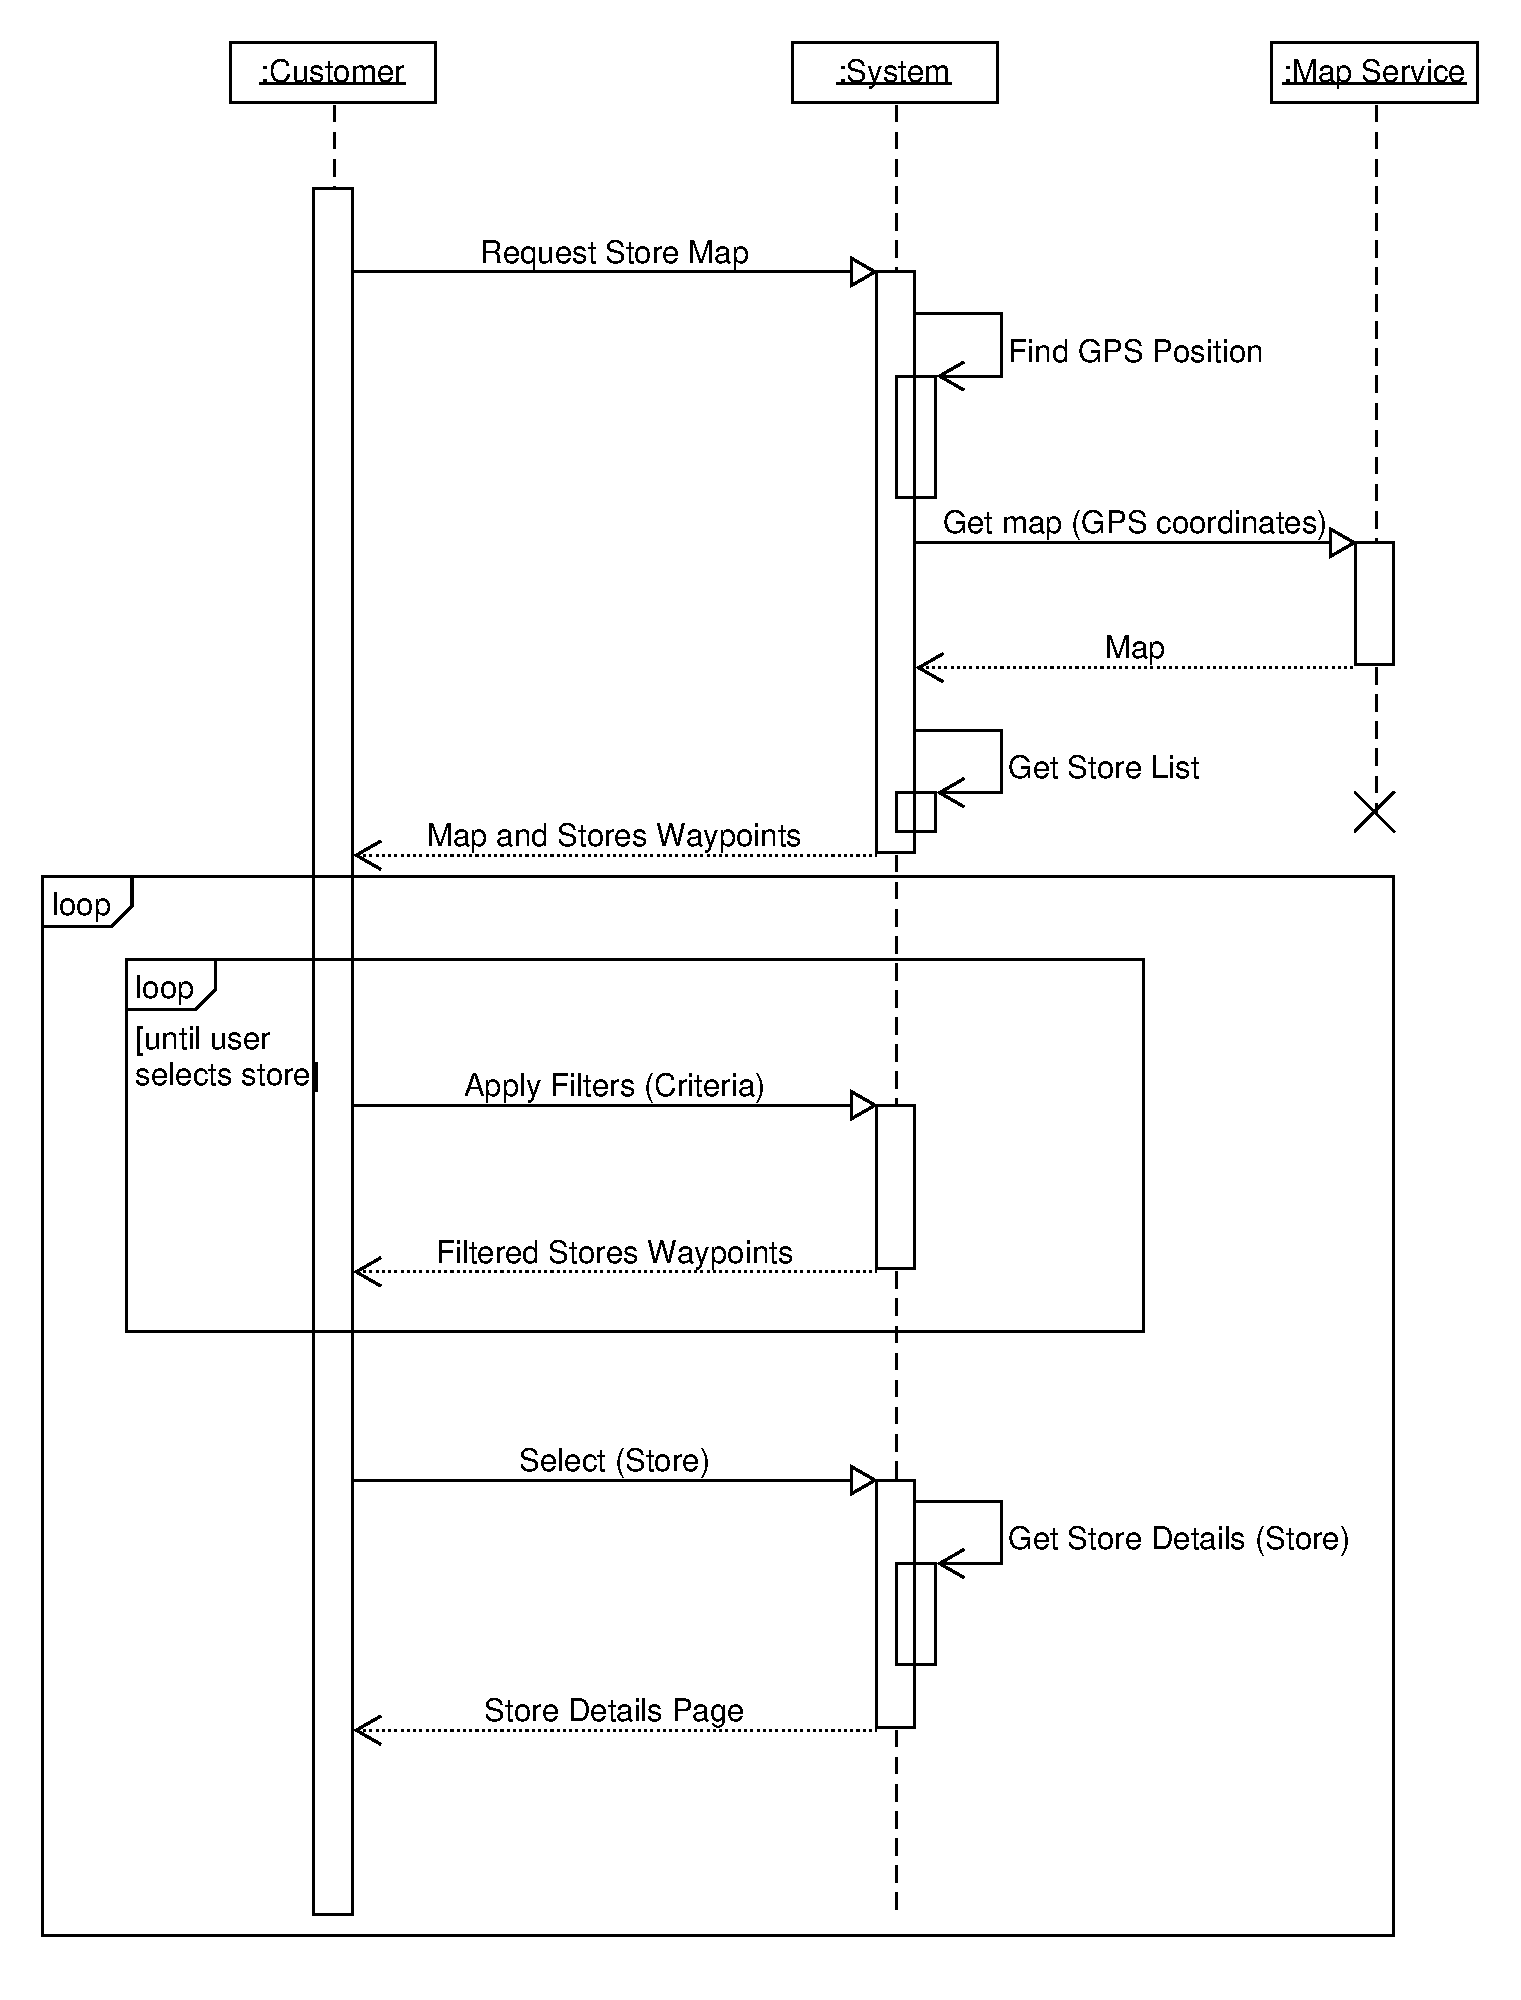
\includegraphics[width=\textwidth]{Images/UML_Seq_Diag_3_2.pdf}
    \caption{\label{fig:Use_Case_Diag}Sequence Diagram for Use Case 3}
\end{figure}

\clearpage
\textbf{Use case 4: Customer adds/removes a store from their favorites list}
\smallskip
\rowcolors{1}{white}{white}
\begin{longtable}{p{0.25\linewidth}p{0.75\linewidth}}
    \toprule
    \textbf{Name}             & \textbf{Customer adds/removes a store to their favorites list} \\
    \midrule
    \textbf{Actors}           & Registered customer                                            \\
    \midrule
    \textbf{Entry conditions} & The user is authenticated and has loaded a store view          \\
    \midrule
    \textbf{Flow of events}   &
    \begin{enumerate}
        \item The user clicks on the button to add/remove the store from the favorites
        \item If the store is on the user's favorites list the store is removed from that list; else the store is added to that list
    \end{enumerate}                                                                 \\
    \midrule
    \textbf{Exit conditions}  & The user sees the change on their favourite list               \\
    \midrule
    \textbf{Exceptions}       &                                                                \\
    \bottomrule
    \caption{\emph{Customer adds/removes a store to their favorites list} use case description}
\end{longtable}


\clearpage
\textbf{Use case 5: Customer books a visit in a store}
\smallskip
\rowcolors{1}{white}{white}
\begin{longtable}{p{0.25\linewidth}p{0.75\linewidth}}
    \toprule
    \textbf{Name}             & \textbf{Customer books a visit in a store}                                                                                  \\
    \midrule
    \textbf{Actors}           & Registered customer                                                                                                         \\
    \midrule
    \textbf{Entry conditions} & The user is authenticated and has loaded a store view. The user has no other visits or ticket active                        \\
    \midrule
    \textbf{Flow of events}   &
    \begin{enumerate}
        \item The user starts the procedure selecting the option to book a visit from the store page
        \item The user selects a date
        \item The system retrieves the time slots with at least one free bookable slot and shows them to the user
        \item The user selects his preferred slots sending the information to the System
        \item The systems checks if the slot is currently available, asks the user to select the expected duration of his visit, showing to them a default value
        \item The user (optionally) edits the value and then confirm the booking
        \item The system confirms the booking of the visit
        \item The system asks the customer if they want to \textbf{create a shopping list}
    \end{enumerate}                                                                                                                              \\
    \midrule
    \textbf{Exit conditions}  & The user can enter the store during the booked time-slot                                                                  \\
    \midrule
    \textbf{Exceptions}       & If the selected slot is not available anymore, the system will show an error message inviting the customer to select another available slot \\
    \bottomrule
    \caption{\emph{Customer books a visit in a store} use case description}
\end{longtable}

\begin{figure}[H]
    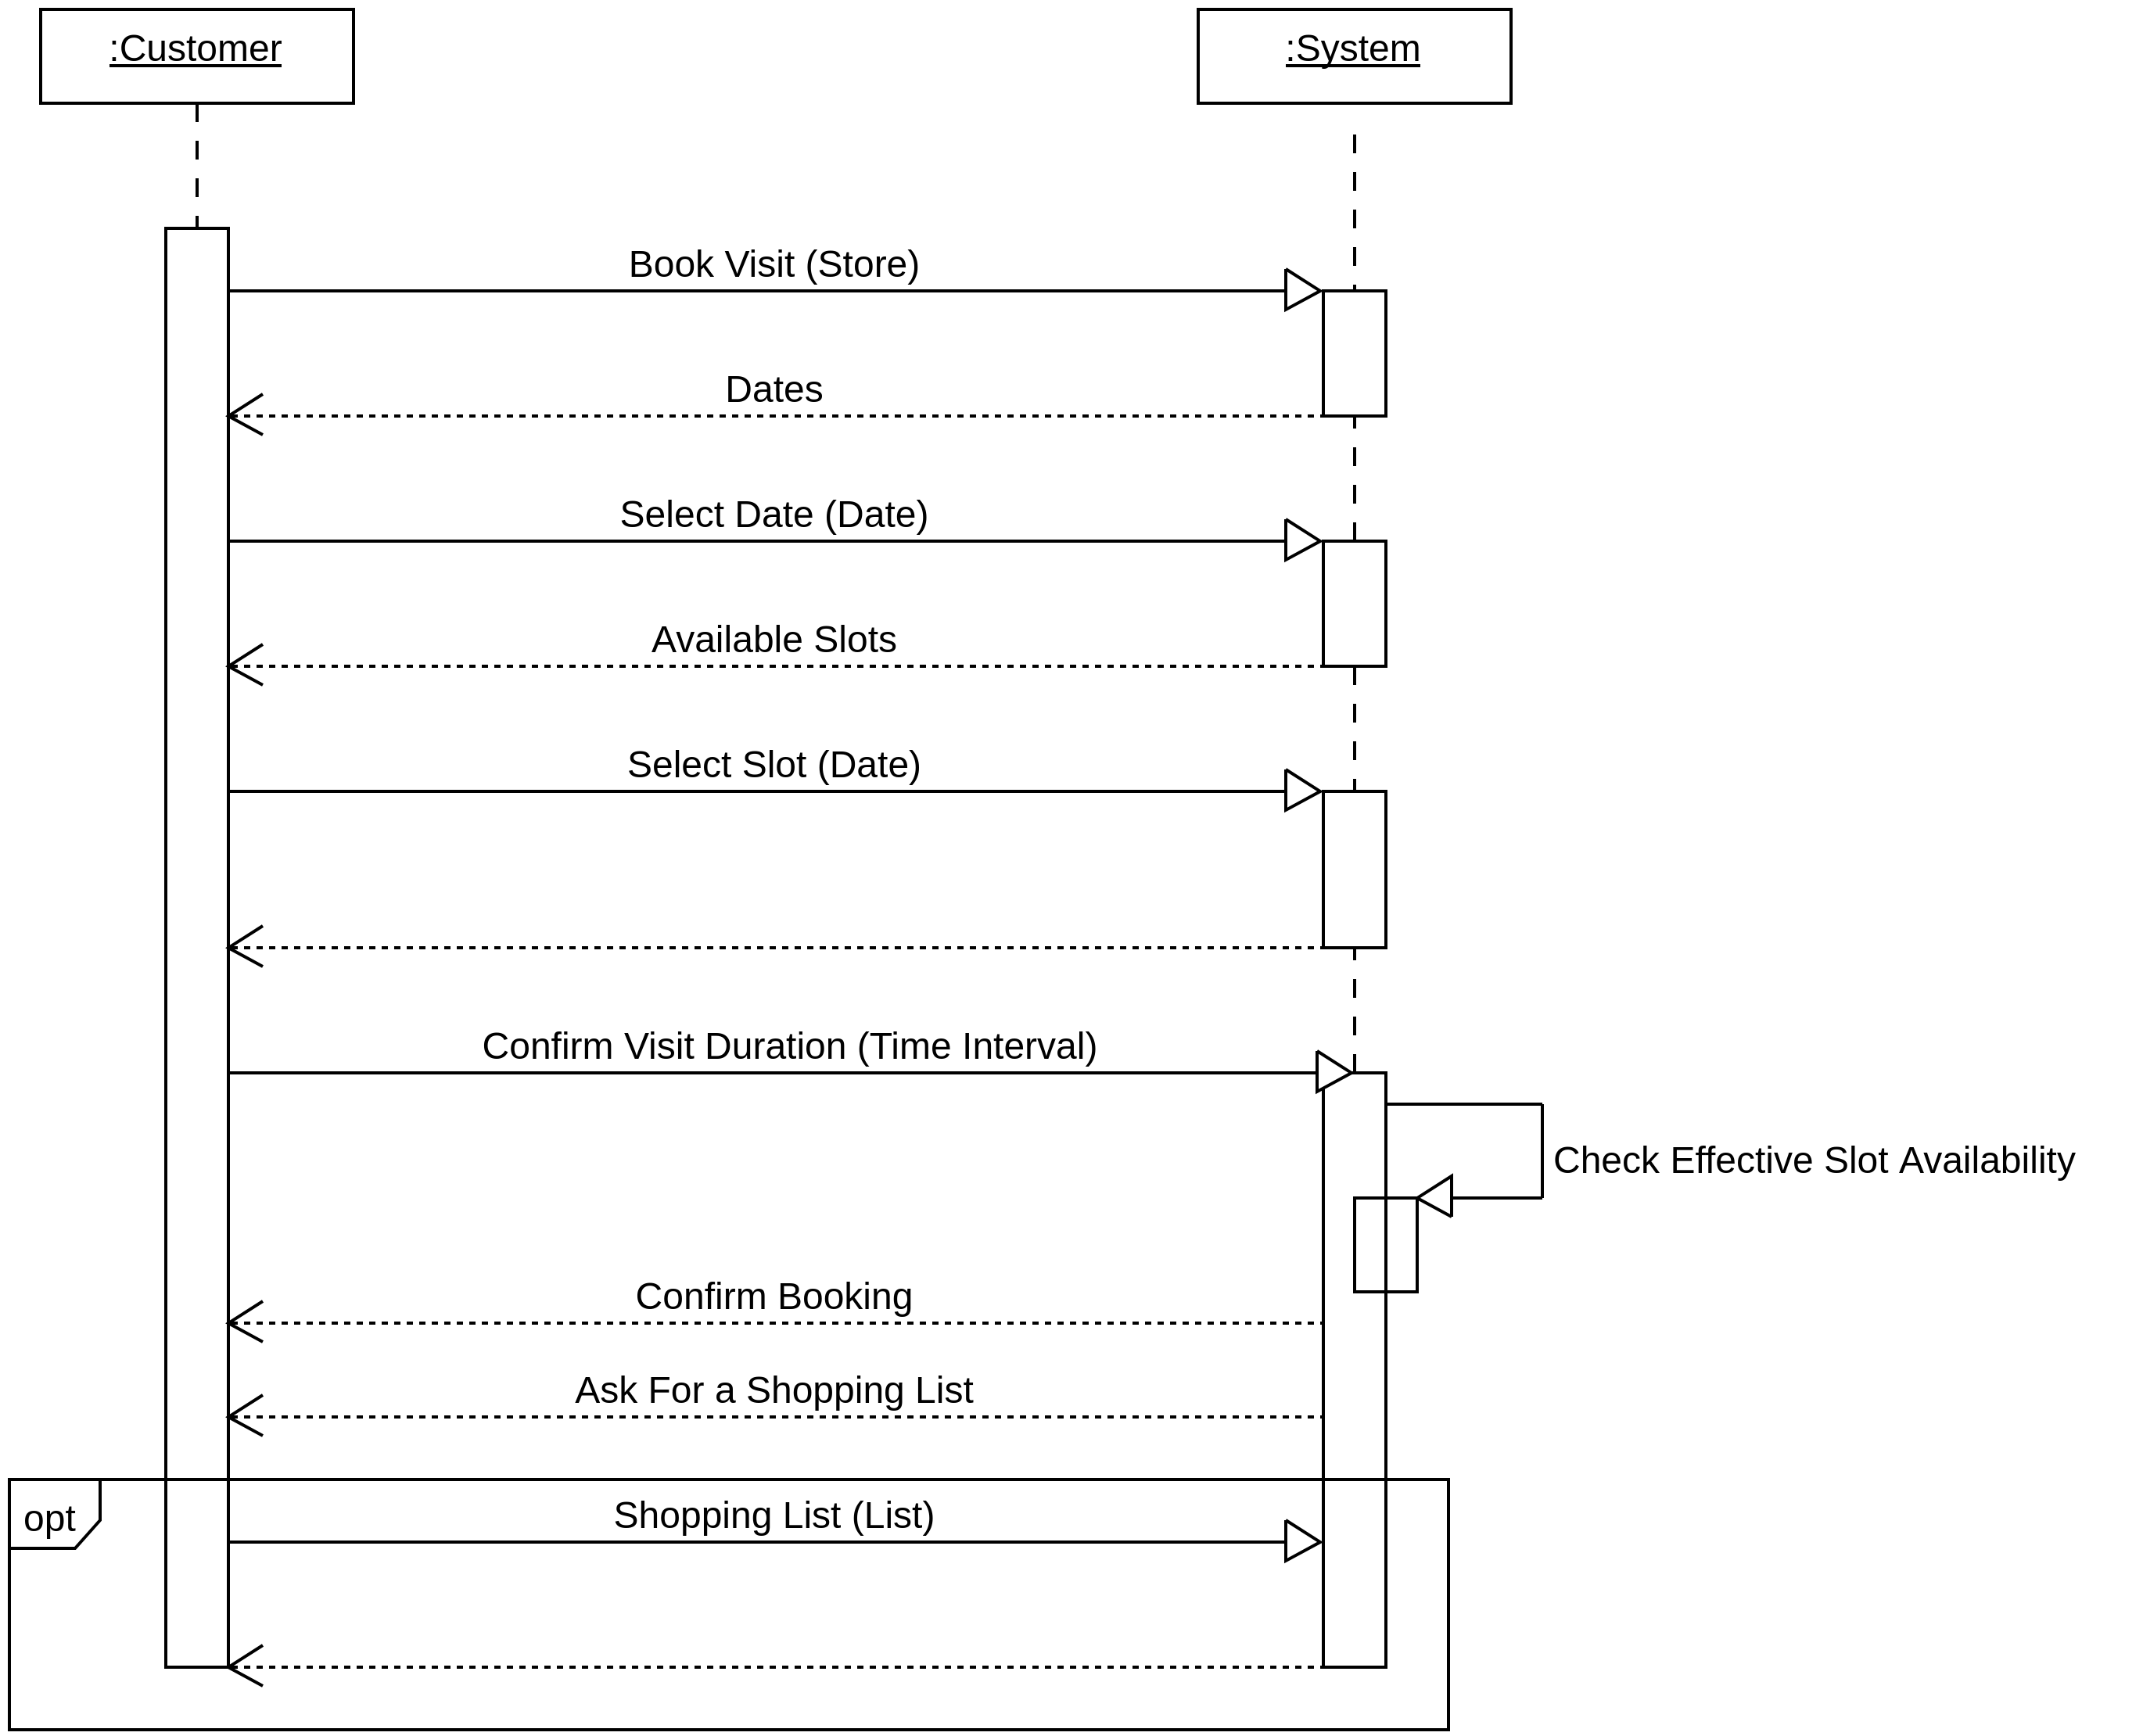
\includegraphics[width=\textwidth]{Images/UML_Seq_Diag_5.png}
    \caption{\label{fig:Use_Case_Diag}Sequence Diagram for Use Case 5}
\end{figure}


\clearpage
\textbf{Use case 6: Customer creates/edits a shopping list}
\smallskip
\rowcolors{1}{white}{white}
\begin{longtable}{p{0.25\linewidth}p{0.75\linewidth}}
    \toprule
    \textbf{Name}             & \textbf{Customer creates/edits a shopping list} \\
    \midrule
    \textbf{Actors}           & Registered customer                             \\
    \midrule
    \textbf{Entry conditions} & The user is authenticated                       \\
    \midrule
    \textbf{Flow of events}   &
    \begin{enumerate}
        \item The user reaches the shopping list view
        \item If the user added a shopping list before, the system asks the user if they want to edit the old list or if they want to start from a blank one
        \item The user inputs a search key in a search bar
        \item The system searches products matching the key and shows them ordered by closeness to the search key
        \item The user choses zero or more than one product from the search results and adds to the shopping list
        \item The user views the complete shopping list and can continue to add or remove product until they confirm the list.
        \item When the user confirms the list, the system will save it in order to make it available to the user the next time they want to compile a shopping list
        \item If the user has booked a visit the system can update the estimates on store departments occupancy on the time of the visit thanks the data on the shopping list
        \item The system acknowledges the user that the list has been saved
    \end{enumerate}                                                  \\
    \midrule
    \textbf{Exit conditions}  &                                                 \\
    \midrule
    \textbf{Exceptions}       &                                                 \\
    \bottomrule
    \caption{\emph{Customer creates/edits a shopping list} use case description}
\end{longtable}

\begin{figure}[H]
    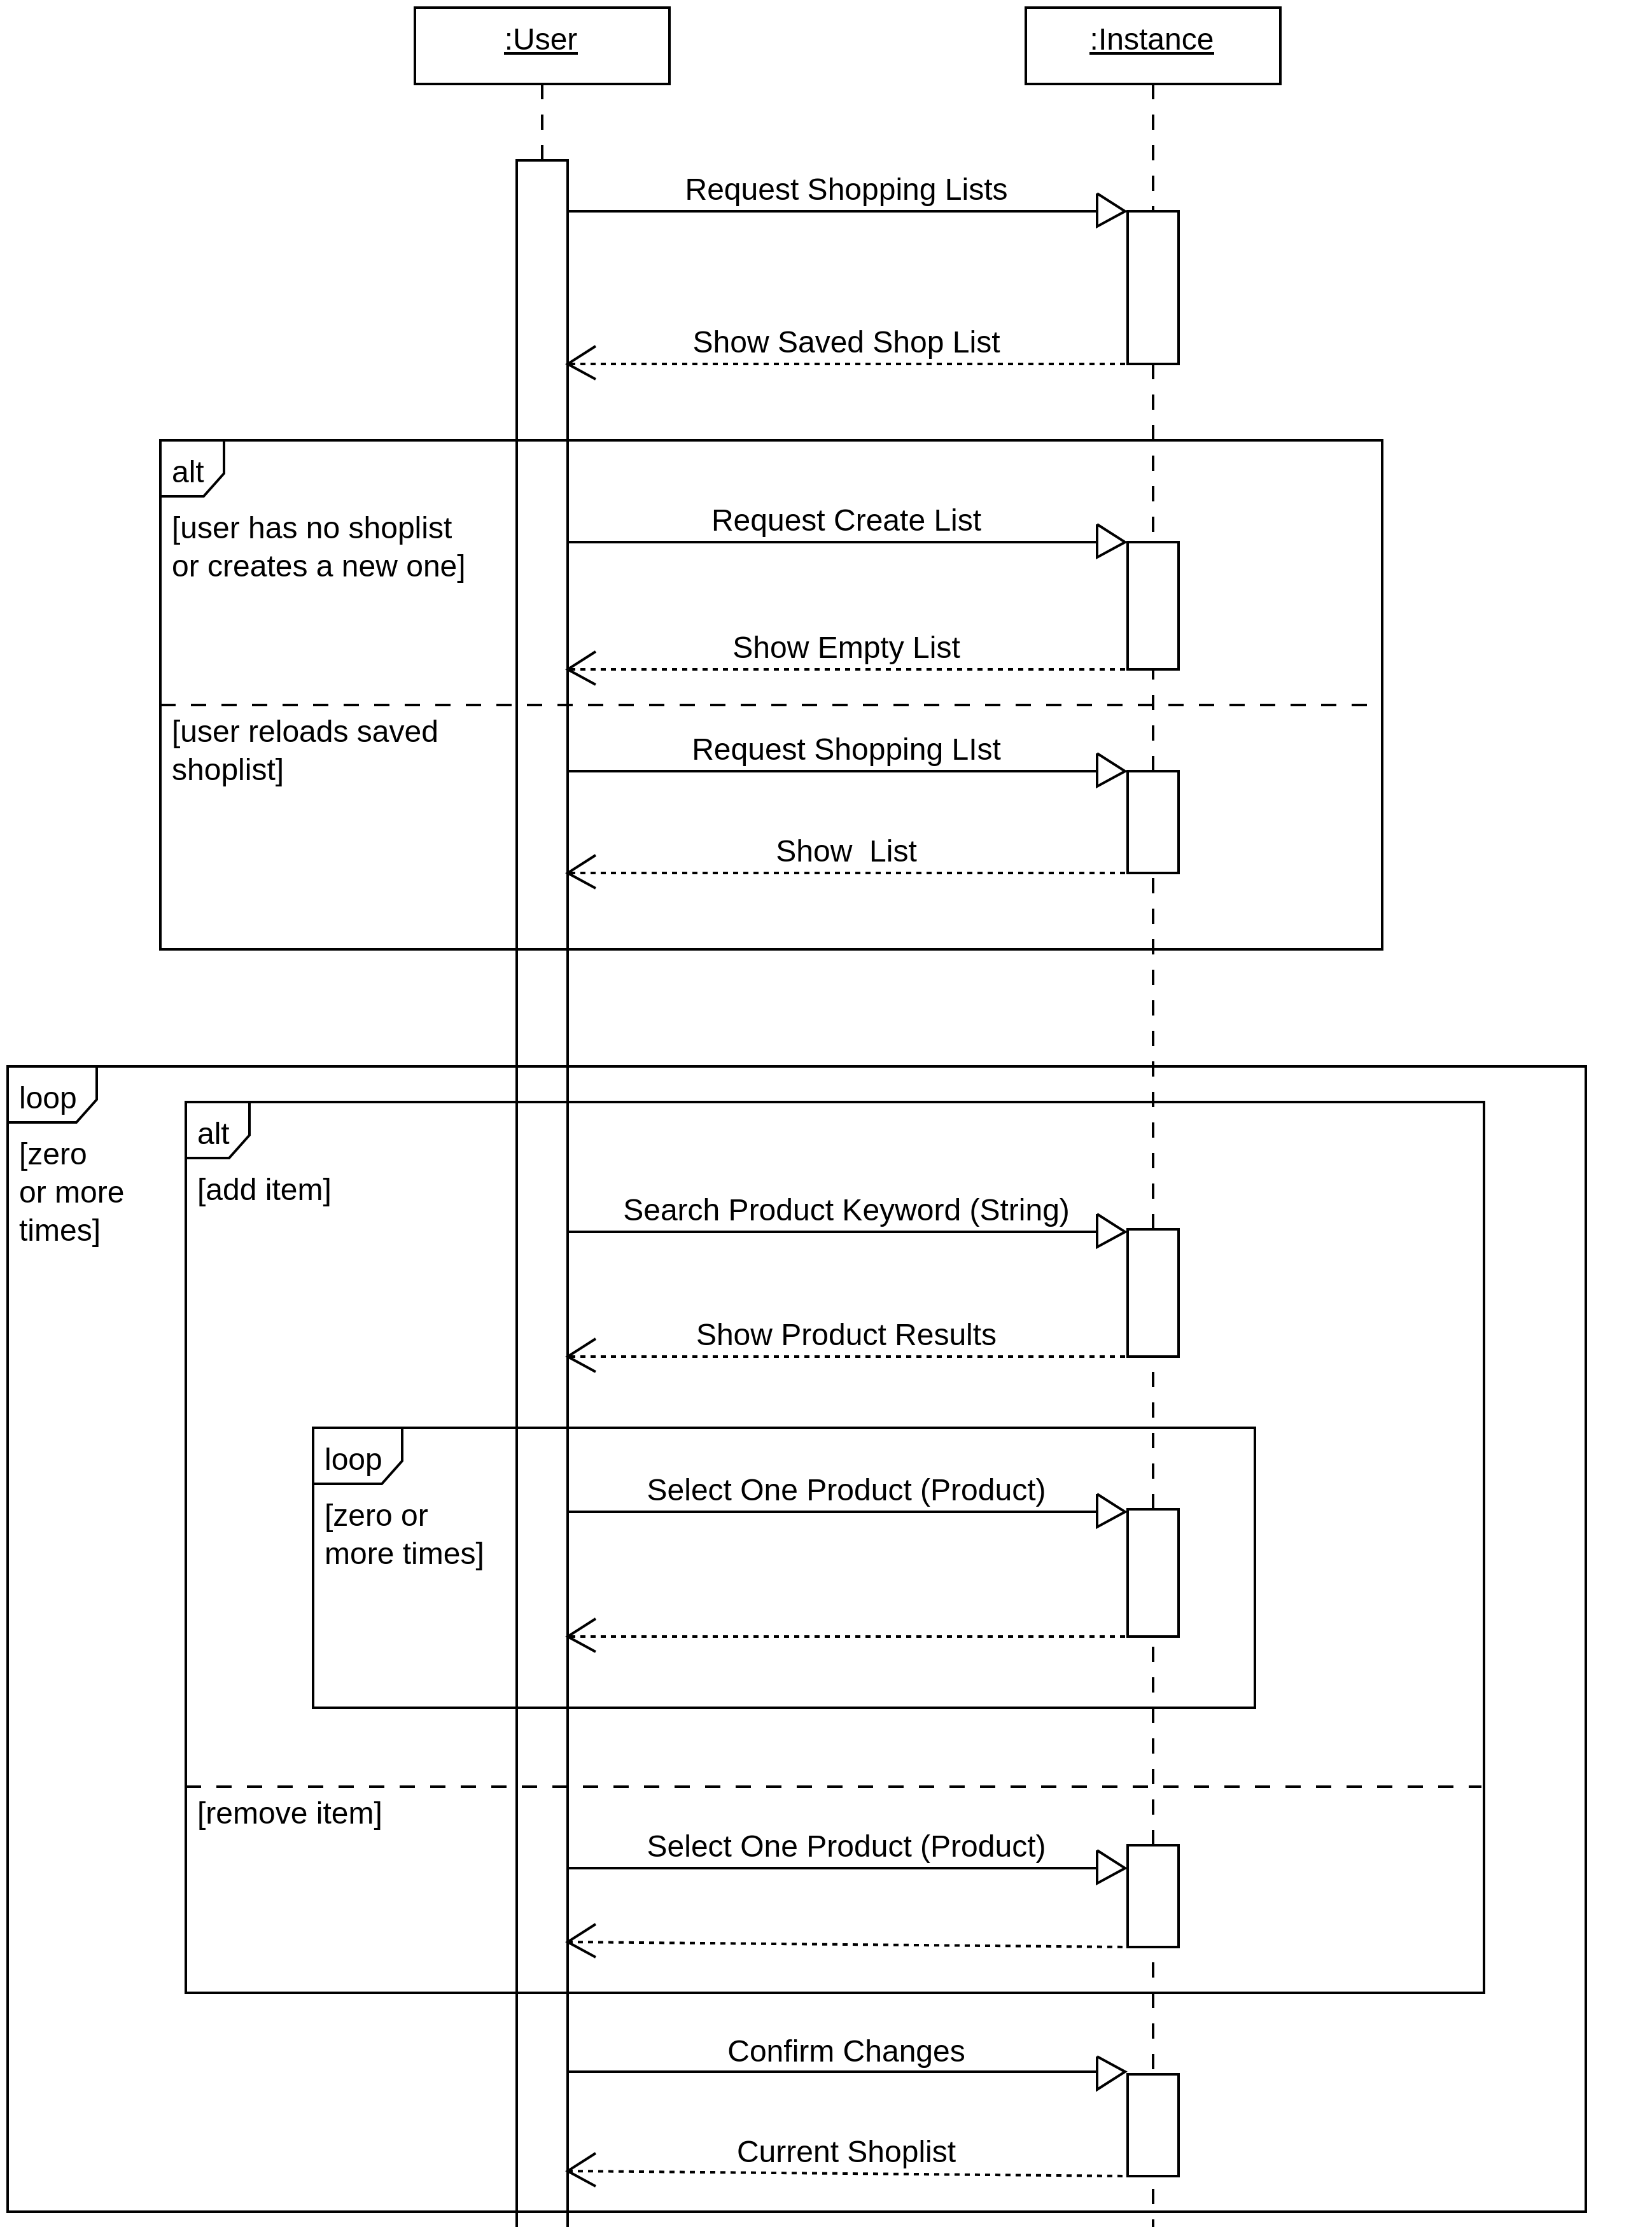
\includegraphics[width=\textwidth]{Images/slice_UML_Seq_Diag_6_1.png}
\end{figure}
\begin{figure}[H]
    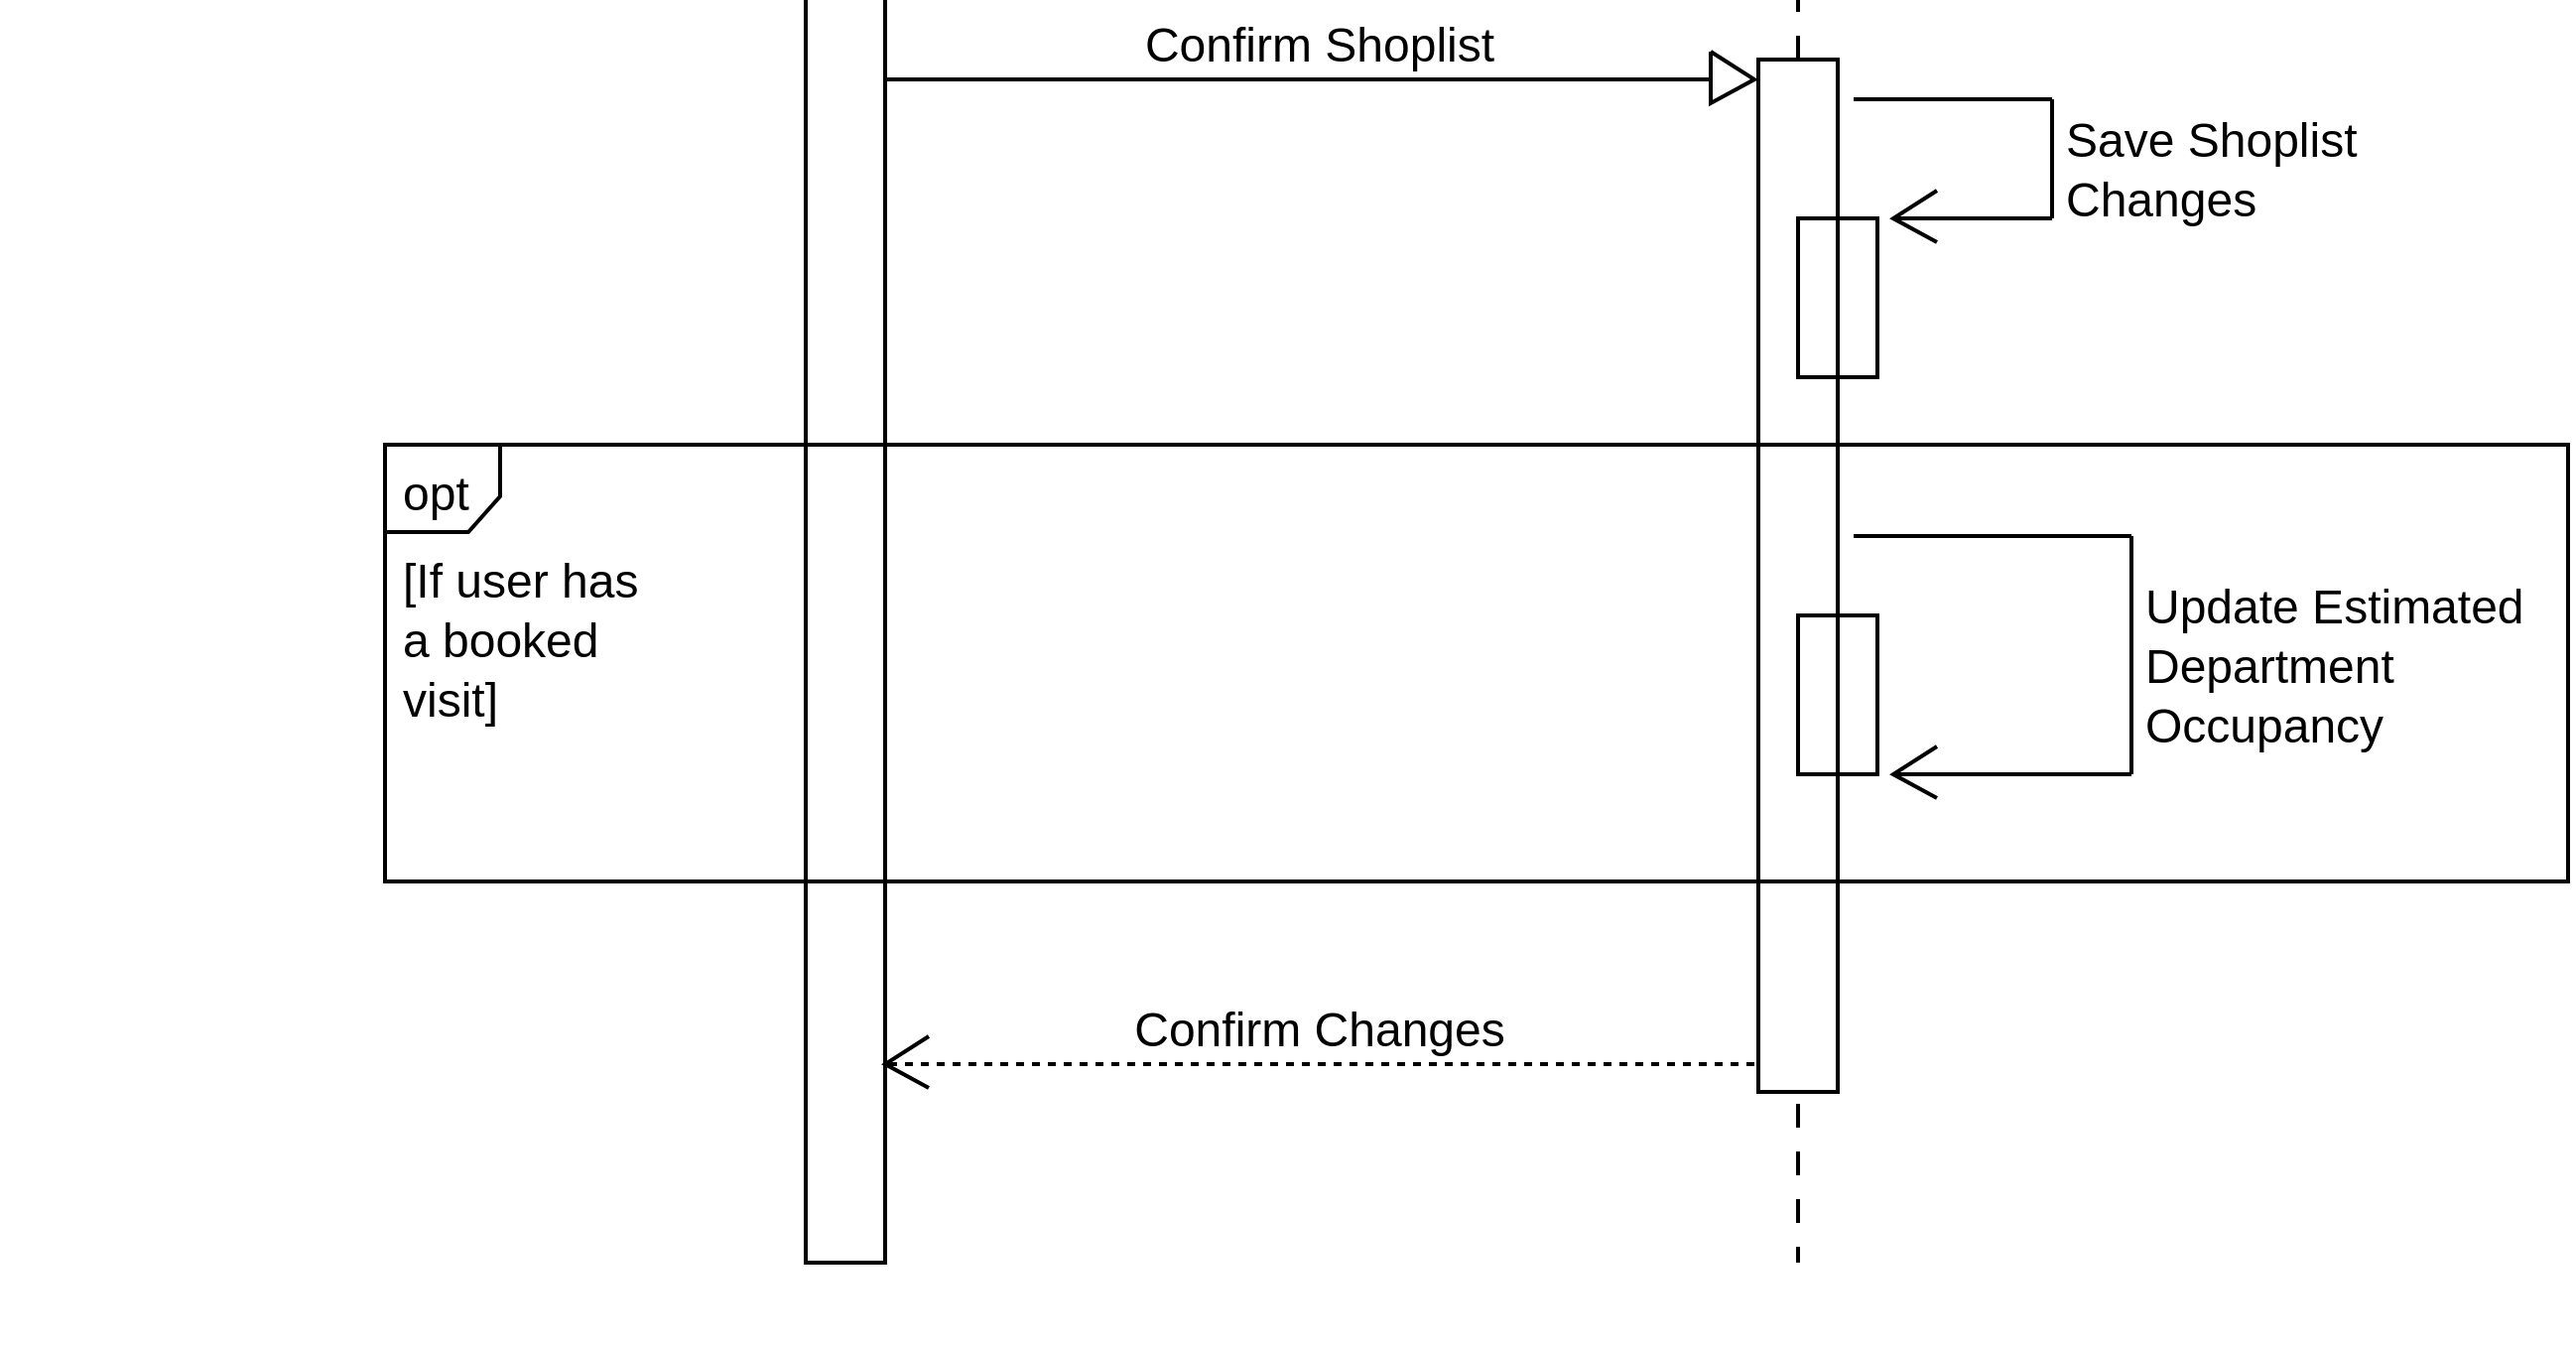
\includegraphics[width=\textwidth]{Images/slice_UML_Seq_Diag_6_2.png}
    \caption{\label{fig:Use_Case_Diag}Sequence Diagram for Use Case 6}
\end{figure}

\clearpage
\textbf{Use case 7: Customer creates a numbered virtual ticket to enter a store as soon as there is place available}
\smallskip
\rowcolors{1}{white}{white}
\begin{longtable}{p{0.25\linewidth}p{0.75\linewidth}}
    \toprule
    \textbf{Name}             & \textbf{Customer create a numbered virtual ticket to enter a store as soon as there is place available} \\
    \midrule
    \textbf{Actors}           & Registered customer                                                                                     \\
    \midrule
    \textbf{Entry conditions} & The user is authenticated and has loaded a store view. The user has no other visits or ticket active    \\
    \midrule
    \textbf{Flow of events}   &
    \begin{enumerate}
        \item The user starts the procedure selecting the option to retrieve a numbered ticket from the store page
        \item The system estimates the waiting time based on the number of people queued and the people actually inside the store
        \item The system confirms the emission of the ticket to the user and shows them the number and other ticket details
        \item If the waiting time changes in a significant way the system notifies the user with the new waiting time
        \item The system alerts the user when it's time to approach the entrance
    \end{enumerate}                                                                                                          \\
    \midrule
    \textbf{Exit conditions}  & The user goes to the entrance and scans the ticket                                                      \\
    \midrule
    \textbf{Exceptions}       &
    \begin{itemize}
        \item If the waiting time is long the system shows an alert to the user asking if they are sure of creating the ticket despite the long queue
        \item If the user takes too long to enter the store after being called to enter an alert is shown stating that the entry is no more guaranteed with that ticket

    \end{itemize}                                                                                                          \\
    \bottomrule
    \caption{\emph{Customer creates a numbered ticket to enter a store as soon as there is place available} use case description}
\end{longtable}

\begin{figure}[H]
    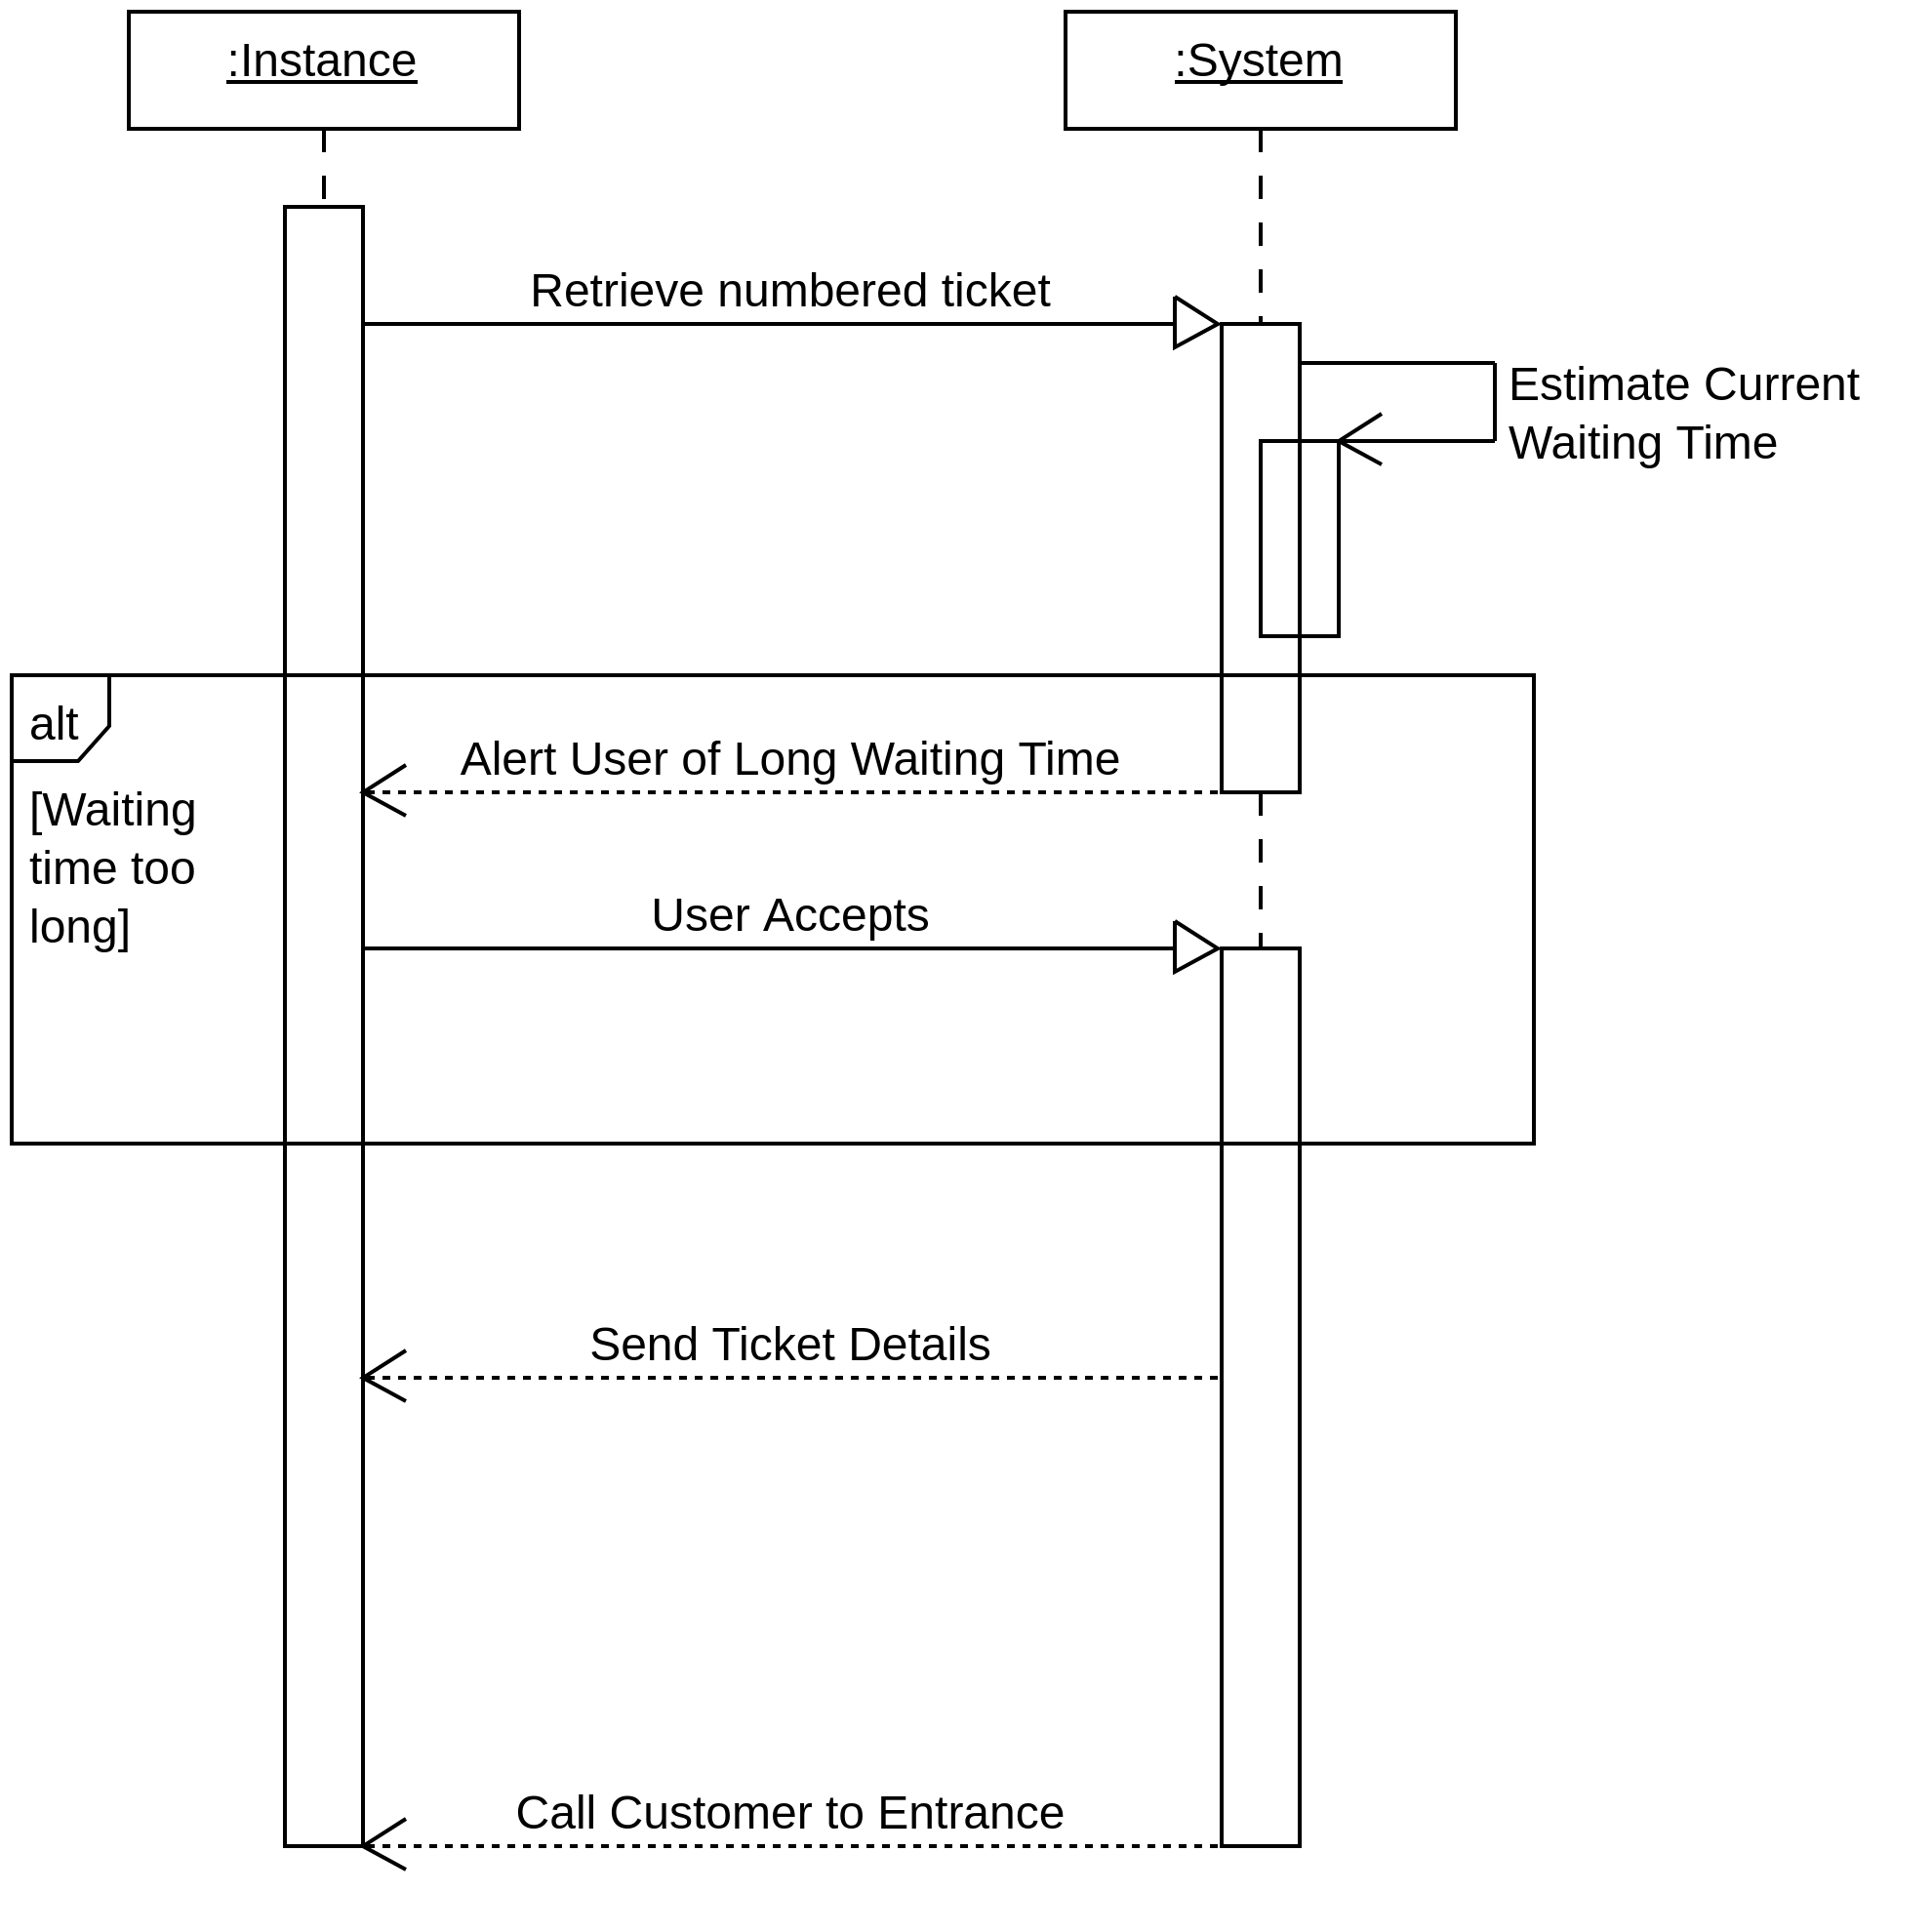
\includegraphics[width=\textwidth]{Images/UML_Seq_Diag_7.png}
    \caption{\label{fig:Use_Case_Diag}Sequence Diagram for Use Case 7}
\end{figure}

\clearpage
\textbf{Use case 8: Customer create a numbered physical ticket to enter the store}
\smallskip
\rowcolors{1}{white}{white}
\begin{longtable}{p{0.25\linewidth}p{0.75\linewidth}}
    \toprule
    \textbf{Name}             & \textbf{Customer create a numbered physical ticket to enter the store}                                                                   \\
    \midrule
    \textbf{Actors}           & Customer, Physical Ticket Emitter                                                                                                        \\
    \midrule
    \textbf{Entry conditions} & The customer is in front of the ticket emitter                                                                                           \\
    \midrule
    \textbf{Flow of events}   &
    \begin{enumerate}
        \item The user selects a button to create a new ticket
        \item The emitter request the system to create a new numbered ticket
        \item The system estimates the waiting time based on the number of people queued and the people actually inside the store
        \item The system returns the details of the ticket to the emitter
        \item The emitter prints the ticket
        \item The user retrieves the ticket and waits until the number on his ticket is called at the entrance of the store
    \end{enumerate}                                                                                                                                           \\
    \midrule
    \textbf{Exit conditions}  & The user enters the store scanning the ticket                                                                                            \\
    \midrule
    \textbf{Exceptions}       & If the user takes too long to enter the store after being called to enter, the ticket no more guarantees the entrance to the store \\
    \bottomrule
    \caption{\emph{Customer create a numbered physical ticket to enter the store} use case description}
\end{longtable}

\clearpage
\textbf{Use case 9: Customer cancels a previously created ticket}
\smallskip
\rowcolors{1}{white}{white}
\begin{longtable}{p{0.25\linewidth}p{0.75\linewidth}}
    \toprule
    \textbf{Name}             & \textbf{Customer cancels a previously created ticket}                                      \\
    \midrule
    \textbf{Actors}           & Registered Customer                                                                        \\
    \midrule
    \textbf{Entry conditions} & The customer has a visit to a store booked or a numbered virtual ticket previously created \\
    \midrule
    \textbf{Flow of events}   &
    \begin{enumerate}
        \item The customer from the virtual ticket/booking view selects the option to cancel the ticket/booking
        \item The system deletes the item from the database and triggers a reevaluation of the estimations about the occupancy of the store and the departments
        \item The system acknowledges the user that the operation was successful
    \end{enumerate}                                                                                             \\
    \midrule
    \textbf{Exit conditions}  & The user can now create another ticket or book another visit                             \\
    \midrule
    \textbf{Exceptions}       &                                                                                            \\
    \bottomrule
    \caption{\emph{Customer cancels a previously created ticket} use case description}
\end{longtable}





\clearpage
\textbf{Use case 10: Customer scans the ticket on an access control system to enter the store}
\smallskip
\rowcolors{1}{white}{white}
\begin{longtable}{p{0.25\linewidth}p{0.75\linewidth}}
    \toprule
    \textbf{Name}                               & \textbf{Customer scans the ticket on an access control system to enter the store} \\
    \midrule
    \textbf{Actors}                             & Customer, Access Control System                                                   \\
    \midrule
    \textbf{Entry conditions}                   & The customer has a ticket or a visit reservation                                  \\
    \midrule
    \textbf{Flow of events}                     &
    \begin{enumerate}
        \item The user scans the machine readable identifier on the ticket at the Access Control System
        \item The access control system sends the scanned ticket identifier to the system
        \item The system determines if the customer can enter, retrieving information about the ticket and the current occupancy of the supermarket
        \item The system sends a confirmation to the Access Control System
        \item The Access Control System lets the customer enter
    \end{enumerate}                                                                                                      \\
    \midrule
    \textbf{Exit conditions}                    & The user is inside the store                                                      \\
    \midrule
    \textbf{Exceptions}                         &
    \begin{itemize}
        \item If the Access Control System fails to recognize the ticket identifer, the user will be asked to scan again the ticket
        \item If the ticket is not valid, the Access Control System won't let the customer enter. This decision can be overridden by an human operator if the system is manned
        \item If the supermarket occupancy is over the legal capacity, the access control won't let the customer enter even with a valid ticket. The system will ask the customer to wait and will consider the booking of the current time slot valid also after the expiration
        \item If the Access Control System fails to communicate with the system, the customer is asked to scan again the ticket and if fails again asks the customer to notify the store personnel (only if the system is not manned).
    \end{itemize}                                                                                                      \\
    \bottomrule
    \textbf{Additional \linebreak Requirements} &
    \begin{itemize}
        \item A booked ticket is valid only in the booked date within the time slot indicated in the ticket.
        \item A numbered ticket is valid only for a limited time after the ticket number has been called to the entrance.
        \item All the tickets are bound to a specific store and could be used only on that store.
        \item The store can allow customer to enter with an expired ticket if the store is far from being full.
    \end{itemize}                                                                                                      \\
    \bottomrule
    \caption{\emph{Customer scans the ticket in an access control system to enter the store} use case description}
\end{longtable}

\begin{figure}[H]
    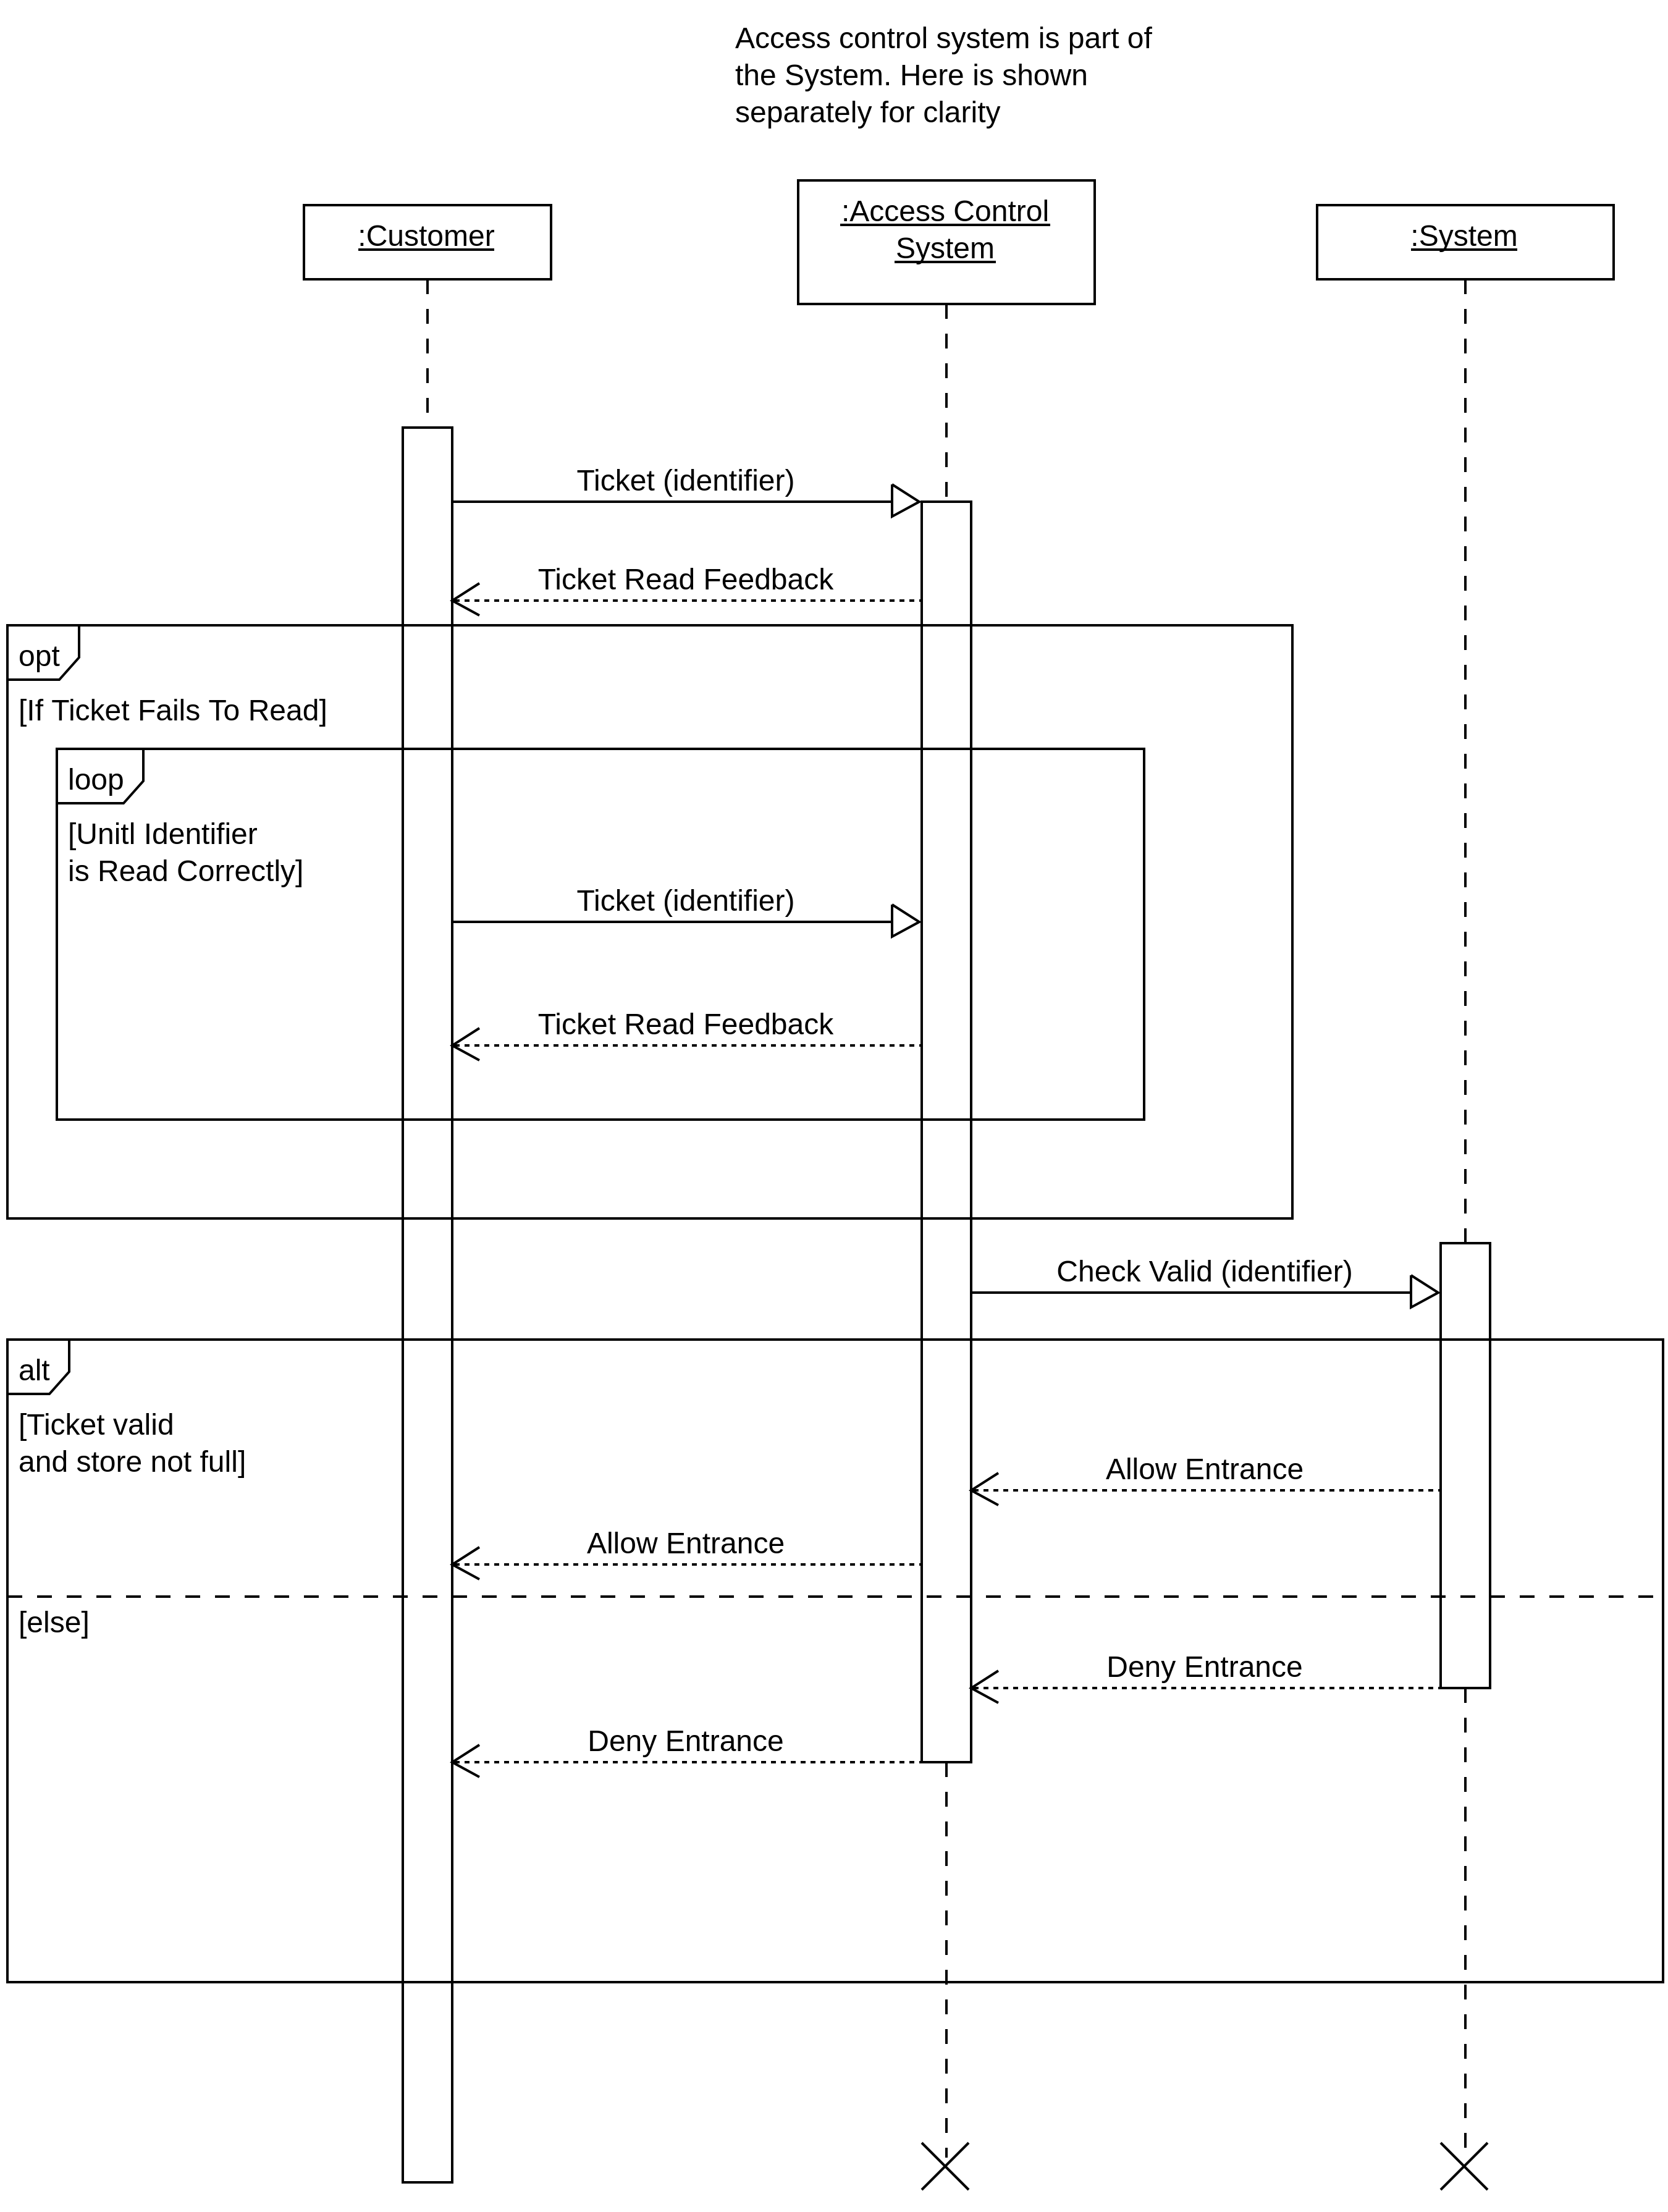
\includegraphics[width=\textwidth]{Images/UML_Seq_Diag_10.png}
    \caption{\label{fig:Use_Case_Diag}Sequence Diagram for Use Case 10}
\end{figure}

\clearpage
\textbf{Use case 11: An user leaves the store through an exit with a people counter installed}
\smallskip
\rowcolors{1}{white}{white}
\begin{longtable}{p{0.25\linewidth}p{0.75\linewidth}}
    \toprule
    \textbf{Name}             & \textbf{An user leaves the store through an exit with a people counter installed}    \\
    \midrule
    \textbf{Actors}           & Customer, People Counter                                                             \\
    \midrule
    \textbf{Entry conditions} & The customer is inside the store                                                     \\
    \midrule
    \textbf{Flow of events}   &
    \begin{enumerate}
        \item The customer walks out of the store through a gate with a people counter installed
        \item The people counter registers that a person passed through the gate
        \item The people counter contacts the system, updating the occupancy real time information
    \end{enumerate}                                                                                       \\
    \midrule
    \textbf{Exit conditions}  & The customer is out of the store and the count of the people of the store is updated \\
    \midrule
    \textbf{Exceptions}       &                                                                                      \\
    \bottomrule
    \caption{\emph{An user exits the store through an exit with a people counter installed} use case description}
\end{longtable}

\clearpage
\textbf{Use case 12: A store operator checks statistics about the store}
\smallskip
\rowcolors{1}{white}{white}
\begin{longtable}{p{0.25\linewidth}p{0.75\linewidth}}
    \toprule
    \textbf{Name}             & \textbf{A store operator checks statistics about the store}                                        \\
    \midrule
    \textbf{Actors}           & Store Operator/ Store Manager                                                                      \\
    \midrule
    \textbf{Entry conditions} & The Store Operator/Store Manager is authenticated                                                  \\
    \midrule
    \textbf{Flow of events}   &
    \begin{enumerate}
        \item The store operator requires to see statistics or real time information about the store collected by CLup
        \item The system retrieves or compute that information
        \item The system present the data to the Operator/Manager
    \end{enumerate}                                                                                                     \\
    \midrule
    \textbf{Exit conditions}  & The Operator/System can now see the data presented by the System                                   \\
    \midrule
    \textbf{Exceptions}       & The system throws an error to the operator if he has no privilege to see the requested information \\
    \bottomrule
    \caption{\emph{A store operator checks statistics about the store} use case description}
\end{longtable}

\clearpage
\textbf{Use case 13: User resets the password}
\smallskip
\rowcolors{1}{white}{white}
\begin{longtable}{p{0.25\linewidth}p{0.75\linewidth}}
    \toprule
    \textbf{Name}             & \textbf{A store operator checks statistics about the store} \\
    \midrule
    \textbf{Actors}           & Registered Customer/ Store Manager                          \\
    \midrule
    \textbf{Entry conditions} & The user  requests a password reset                         \\
    \midrule
    \textbf{Flow of events}   &
    \begin{enumerate}
        \item The user inputs his e-mail
        \item The system checks that the e-mail corresponds to a registered account
        \item The system sends an e-mail to the user with a temporary link to the reset password page
        \item The user opens the link and inputs his new password
        \item The user confirms his new password
        \item The system applies the changes and redirects the user to the proper login page
    \end{enumerate}                                                              \\
    \midrule
    \textbf{Exit conditions}  & The password of the user account is changed                 \\
    \midrule
    \textbf{Exceptions}       &
    \begin{itemize}
        \item If the e-mail inserted from the user is not associated with any of the accounts an error message is shown to the user.
        \item While typing the password the system checks that the password is compliant with the password requirements listed in the section \ref{password_req}. If the password requirements are not met the system shows an error listing the non respected password requirements.
    \end{itemize}                                                              \\
    \bottomrule
    \caption{\emph{User resets the password} use case description}
\end{longtable}
\clearpage

\subsubsection{Requirements Mapping}
In this sections each goal is mapped to the functional requirements and the domain assumptions that combined satisfy that goal. Each goals also includes the use cases involved from that goal.
\bigskip
\begin{itemize}
    \item \textbf{G1 Avoid exceeding the maximum number of customer inside the store in each store}
    \begin{itemize}
        \item R1 The system must keep general information and contacts about the store chains adopting CLup
        \item R2 The system must provide each store a store-admin account
        \item R3 The store-admin account must allow the creation of store-operator accounts
        \item R4 For each store the system must allow the users to retrieve information about location and business hours
        \item R5 The system stores information about capacity of each market
        \item R6 The system won’t let anyone enter the store if the maximum capacity has been reached
        \item R7 The system will let a customer enter the store if and only if he has a a valid ticket
        \item R8 The system will use the occupancy data retrieved from the store to control the store access
        \item R9 The system must provide an interface to communicate with the store access control
        \medskip
        \item DA2 Customer will stay approximately the time they have declared when booking the ticket
        \item DA3 The access controller works properly and won't allow unauthorized customers entrances
        \item DA6 If people counters are installed they will provide the exact count of the customers that enter or leave the shop
        \item DA7 No customer are present at the shop opening hour, and no customer will be present at the shop closing hour
        \item DA8 The store manager will insert correct data about the shop and the departments maximum capacities
        \medskip
        \item UC10 Customer scans the ticket through an access control system to enter
        \item UC11 An user leaves the store through an exit with a people counter installed
    \end{itemize}
    \item \textbf{G2 Reduce the number of customer waiting physically in line in front of the store entrance}
    \begin{itemize}
        \item R12 The system must allow the store-admin account to create and edit entrance time intervals
        \item R13 Each time interval must have a number of bookable slots fewer than the store capacity
        \item R14 The system must allow authenticated users to book a visit in a desired time interval
        \item R17 The system must allow a customer to create a numbered virtual queue ticket and notify them if he can enter immediately (if the store is not full) or provide them a waiting time estimation
        \item R18 The system must notify the customers with a virtual queue ticket when it’s time to approach the store entrance
        \item R19 The store operator application must allow an authenticated Notify a customer with the CLup app a reasonably precise estimation of the waiting time
        \item DA4 Customers with a numbered digital ticket try to avoid staying near the entrance until they receive the “go to entrance” notification
        \item DA5 Customers with a booked ticket in a given time slot will not show up until few minutes before the start of their time slots
        \medskip
        \item UC5 Customer books a visit in a store
        \item UC7 Customer creates a numbered virtual ticket to enter a store as soon as there is a place available
    \end{itemize}
    \item \textbf{G3 Try to distribute people uniformly inside the store to ease maintaining social distancing}
    \begin{itemize}
        \item R10 The system must provide an interface for user to compile a shopping list    
        \item R11 The system must take in consideration shopping list data and historic data from previous user visits to reduce store crowdedness per department
        \item R36 The system allows customer to register an user account
        \item R37 The system allows registered customers to authenticated
        \medskip
        \item DA1 Customers that created a shop list will buy approximately all the products in that list, so they will visit for the greater part of their permanence the departments where the products are located
        \item DA2 Customer will stay approximately the time they have declared when booking the ticket
        \medskip
        \item UC6 Customer creates/edits a shopping list
    \end{itemize}
    \item \textbf{G4 Allow customers to book for a visit to the store at a desired time and day}
    \begin{itemize}
        \item R12 The system must allow the store-admin account to create and edit entrance time intervals
        \item R13 Each time interval must have a number of bookable slots fewer than the store capacity
        \item R14 The system must allow authenticated users to book a visit in a desired time interval
        \item R15 The system must not allow a user to book a slot in an already full time interval
        \item R16 The system must not allow a user to book a visit if he has already reserved another visit
        \item R20 The system  must ask the customer to provide the estimated visit time when booking a visit to the store
        \item R30 The stores adopting CLup must be displayed on a map
        \item R32 The CLup customer app allows to book visit and retrieve tickets directly from the store page
        \item R36 The system allows customer to register an user account
        \item R37 The system allows registered customers to authenticated
        \medskip
        \item DA7 No customer are present at the shop opening hour, and no customer will be present at the shop closing hour
        \item DA8 The store manager will insert correct data about the shop and the departments maximum capacities
        \medskip
        \item UC1 Customer Registration
        \item UC2 Customer/Operator Authentication
        \item UC3 Customer search for the store page
        \item UC5 Customer books a visit in a store
        \item UC9 Customer cancels a previously created 
        ticket
        \item UC10 Customer scans the ticket through an access control system to enter
        \item UC13 User resets his password
    \end{itemize}
    \item \textbf{G5 Let every customer have the possibility to access the store regardless of the technology available to them}
    \begin{itemize}
        \item R21 The system must allow stores to hand out numbered physical queueing tickets to those that do not use the CLup application
        \item R22 The system must allow the access to the store to customer with numbered tickets using a ’First Come First Served’ logic, treating virtual and physical tickets owner equally
        \item R23 The system must try to estimate waiting time based on store capacity, reservations and the current number of people with numbered tickets waiting in line
        \item R24 The system should interface with an screen placed at the entrance of the store to notify customer which ticket numbers will enter in the next called batch
        \item R29 The customer CLup application must be cross-platform and must work on the majority of the devices
        \medskip
        \medskip
        \item UC8 Customer creates a physical numbered ticket
        \item UC10 Customer scans the ticket through an access control system to enter
    \end{itemize}
    \item \textbf{G6 Give stores adopting CLup access to anonymous statistics regarding the people coming to the store}
    \begin{itemize}
        \item R2 The system must provide each store a store-admin account
        \item R3 The store-admin account must allow the creation of store-operator accounts
        \item R25 The system must let the store-admin accounts retrieve statistics collected from CLup regarding their store 
        \item R26 The system must record periodically and store statistics about the occupancy of each store
        \item R27 The customer CLup application must show brief statistics about average occupancy of each stores during different days of the week
        \item R28 The operator CLup application must show to an authenticated operator the real time occupancy of the stor
        \medskip
        \item DA8 The store manager will insert correct data about the shop and the departments maximum capacities
        \medskip
        \item UC2 Customer/Operator Authentication 
        \item UC12 A store operator checks statistics about the store  
    \end{itemize}
    \item \textbf{G7 Provide a simple and user-friendly interface to book tickets}    
    \begin{itemize}
        \item R4 For each store the system must allow the users to retrieve information about location and business hours
        \item R29 The customer CLup application must be cross-platform and must work on the majority of the device
        \item R30 The stores adopting CLup must be displayed on a map
        \item R31 The CLup customer application allows user to mark stores as favorite in order to access them quickly
        \item R32 The CLup customer app allows to book visit and retrieve tickets directly from the store page
        \item R34 The system must push notifications to user devices with update information on the store he has a ticket for
        \item R36 The system allows customer to register an user account
        \item R37 The system allows registered customers to authenticated
        \medskip
        \medskip
        \item UC1 Customer Registration
        \item UC2 Customer/Operator Authentication
        \item UC3 Customer search for the store page
        \item UC4 Customer adds/removes a store from their favorites list 
    \end{itemize}                                                
    \item \textbf{G8 Provide an interface for the access controller to check tickets and monitor the occupancy }
    \begin{itemize}
        \item R2 The system must provide each store a store-admin account
        \item R3 The store-admin account must allow the creation of store-operator accounts
        \item R8 The system must provide an interface to communicate with the store access control
        \item R9 The system must provide an interface to communicate with the store access control
        \item R19 The store operator application must allow an authenticated operator to manually admit customers
        \item R23 The system must try to estimate waiting time based on store capacity,reservations and the current number of people with numbered tickets waiting in line
        \item R28 The operator CLup application must show to an authenticated operator the real time occupancy of the store
        \item R33 The system must provide an interface for automated control devices to communicate to CLup data about store entrances, store leavings and crowdedness in the various departments
        \medskip
        \item DA3 The access-control system works properly and won’t allow unauthorized customer entrances
        \item DA6 If people counters are installed they will provide the exact count of the customers that enter or leave the shop
        \item DA8 The store manager will insert correct data about the shop and the departments maximum capacities
        \medskip
        \item UC10 Customer scans the ticket through an access control system to enter
        \item UC12 A store operator checks statistics about the store
    \end{itemize}     
    \item \textbf{G9 Provide an estimation of the waiting time to every customer that waits in line (physical or virtual)}
    \begin{itemize}
        \item R8 The system will use the occupancy data retrieved from the store to control the store access
        \item R17 The system must allow a customer to create a numbered virtual queue ticket and notify them if he can enter immediately (if the store is not full) or provide them a waiting time estimation
        \item R20 The system must ask the customer to provide the estimated visit time when booking a visit to the store
        \item R21 The system must allow stores to hand out numbered physical queueing tickets to those that do not use the CLup application
        \item R22 The system must allow the access to the store to customer with numbered tickets using a ’First Come First Served’ logic, treating virtual and physical ticket owner equally
        \item R23 The system must try to estimate waiting time based on store capacity, reservations and the current number of people with numbered tickets waiting in line
        \item R24 The system should interface with an screen placed at the entrance of the store to notify customer which ticket numbers will enter in the next called batch
        \item R34 The system must push notifications to user devices with update information on the store he has a ticket for
        \medskip
        \item DA2 Customer will stay approximately the time they have declared when booking the ticket
        \medskip
        \item UC7 Customer creates a numbered virtual ticket to enter a store as soon as there is a place available
        \item UC8 Customer creates a physical numbered ticket
    \end{itemize}
    \item \textbf{G10 Notify a customer when it's time to approach the store entrance}
    \begin{itemize}
        \item R8 The system will use the occupancy data retrieved from the store to control the store access
        \item R17 The system must allow a customer to create a numbered virtual queue ticket and notify them if he can enter immediately (if the store is not full) or provide them a waiting time estimation
        \item R18 The system must notify the customers with a virtual queue ticket when it’s time to approach the store entrance
        \item R21 The system must allow stores to hand out numbered physical queueing tickets to those that do not use the CLup application
        \item R24 The system should interface with an screen placed at the entrance of the store to notify customer which ticket numbers will enter in the next called batch
        \item R35 The system must associates tickets with line numbers
        \medskip
        \item DA2 Customer will stay approximately the time they have declared when booking the ticket
        \item DA6 If people counters are installed they will provide the exact count of the customers that enter or leave the shop
        \medskip
        \item UC7 Customer creates a numbered virtual ticket to enter a store as soon as there is a place available
        \item UC8 Customer creates a physical numbered ticket
    \end{itemize}
\end{itemize}


\subsection{Performance Requirements}
Considering \textbf{CLup customer application} and \textbf{CLup operator application}, an user action that implies a communication with a remote server should take no longer than 5 seconds, from the start of the interaction to the moment when the user receives some feedback. When there is no need to connect to a server, this time should be lower than 1 second. This requirements holds in a context where the underlying operative system is not overloaded and the user internet connection is working properly.
\smallskip
When a store admin account requests elaborate statistics of the store, the response time must be lower than 10 seconds.
\subsection{Design Constraints}

\begin{itemize}
    \item General Data Protection Regulation (GDPR, EU 2016/679) must be followed in order to collect data from users.
\end{itemize}

\subsection{Software System Attributes}
\subsubsection{Reliability}
All the data stored in the CLup databases must be periodically backed up. Data redundancy policies, like RAID, must be enacted to hande failures promptly and lowering the risk of losing data.

\subsubsection{Availability}
The system must have multiple nodes handling requests from the customers and the operators. These nodes, working in parallel, reduce the risk of a total failure of the system. Data redundancy policies also help to reduce downtimes in case of a data storage unit fault.

\smallskip

The system uptime should be as close as possible to 100\%. Since that is impossible, an uptime of 99.9\% is more than acceptable and corresponds to less than 9 hours of down time every 365 days.
Ordinary maintenance that needs shutting down part of the system should be planned, if possible, during nights; in this way it is more likely that the majority of the users won't experience disruptions in the use of CLup services.

\smallskip

The access control system must continue working even if an automated, external system installed in the store fails. In the following table are listed the measures that must be taken after a failure of an external system:
\smallskip

\rowcolors{2}{gray!25}{white}
\captionof{table}{External Systems fails table}
\begin{tabular}{C{5cm}L{10.0cm}C{2.0cm}}
    \rowcolor{gray!50}
    External System that fails & Measures                                                                                                                                        \\
    People counter             & The CLup system will estimate the number of people inside the store using the average visit times. This value will also be manually adjustable  \\
    Smart Gates                & An operator with the CLup operator application will check tickets and admit people manually                                                     \\
    Paper Ticket Emitter       & An operator will form a queue and admits people manually if there is space in the store (information that can still be tracked by the CLup app) \\
    Ticket number screens      & An operator announces manually the ticket numbers of the people that should enter the store, looking them up on the CLup operator app           \\
\end{tabular}
\subsubsection{Security}
All the data sent via insecure communication channels (i.e. Internet, Local Networks) must be secured with modern encryption standards. This requirement applies to all data exchanged by CLup customer and operator applications and for all traffic generated by the external hardware systems installed on the store.

\smallskip

The external hardware systems installed in the store should be connected in a secure and dedicated LAN with a single access point to the internet with proper firewall settings. This network must be separated from other networks especially the ones accessible freely from the customers (i.e. a shop free Wi-Fi service).

\smallskip

The customer accounts are separated from the business accounts. Each store manager has permissions to manage the operator accounts and has access to all the store data; the manager can decide which account can view which statistics.
\subsubsection{Maintainability}
The system is clearly divided in a lot of independent subsystems that communicate with each other using some interfaces. As long as the interface between different subsystems is preserved, it is possible to maintain and update single subsystems transparently.
\subsubsection{Portability}
\textbf{The CLup customer mobile application} compatibility should cover at least 95\% of the iOS and Android devices. To make CLup even more accessible, a mobile friendly web interface can be provided to the users.

\smallskip

\textbf{The CLup operator application} must be available via a web application. The functionalities needed for the Access Control Staff must also be available on a mobile application that will be installed on devices given to the staff.
\subsection{Other Requirements}
\subsubsection{Required fields for registration}
When a CLup customer creates a CLup customer account, they have to fill a form. Here are specified requirements regarding the information needed to register to CLup. If not otherwise specified every field is compulsory.

\begin{itemize}
    \item First name
    \item Last name
    \item Address, composed of:
          \begin{itemize}
              \item Country
              \item Region/State
              \item Town
              \item CAP
              \item Street and number
              \item Additional address lines (optional)
          \end{itemize}
    \item Gender (optional)
    \item Date of birth
    \item Valid email address
    \item Password, must respect this criteria:\label{password_req}
          \begin{itemize}
              \item Must have at least a digit
              \item Must have at least a lowercase character
              \item Must have at least a special symbol in this list
                    \begin{verbatim}
                *.!@#$%^&(){}[]:;<>,.?/~_+-=|\
                    \end{verbatim}
              \item Must have a number of characters between 8 and 32
          \end{itemize}
\end{itemize}